% !TeX spellcheck = en_US
% !TEX root = ../thesis-example.tex
%
\chapter{From Video to Mixed Reality}
\label{chap:video2mr}

\todo{Needs better sourcing.}

To achieve a real-time rendering environment, as previously mentioned, there 
are two main production cycles. The one discussed in this thesis resolves this 
problem by staying inside one application with multiple render operations per 
frame, the other will be briefly mentioned in the related work section below. 
\newline
The first and most important render cycle is the stereoscopic output of the 
Vive HMD, which has a set frame rate of either 45 or 90 frames per second - 
this is a hard limitation by the providing library, which stalls Unity's 
rendering if a render cycle is above $11ms = 1s / 90$. It is important to have 
consistent performance, otherwise the experience for an actor with the HMD will 
be terribly degraded. This will influence a mixed reality composition, since 
frame rate targets should be evaluated early in production to fit the 
composition environment. Since the render pipeline is mostly affected by GPU 
performance, high fidelity graphics can be achieved with later iterations of 
graphical hardware. Also recent history has shown that different instancing and 
render methods can yield massive performance gains and will likely improve in 
the future of VR\cite{oculus:improv-render:2016}.
\newline
After rendering a stereoscopic image to the HMD another, secondary render cycle 
has to be done on the same frame, which is an in-engine camera inside the 
virtual scene and the relative position of the real-world HMD and real-world 
camera. Since the SteamVR library for the HTC Vive already exposes a 
normalized, synchronized device tracking, it is easily possible to position the 
in-engine camera at an accurate location of the real world capturing device. 
This positional and rotational data is achieved by strapping a HTC Vive 
Controller (or HTC Vive Tracker) to the real world camera and adding another 
transform to the in-engine render camera to allow for an offset, which is 
yielded to the difference between sensor location of the video capturing device 
and the tracking center of a controller / tracker.

\begin{figure}[htb]
	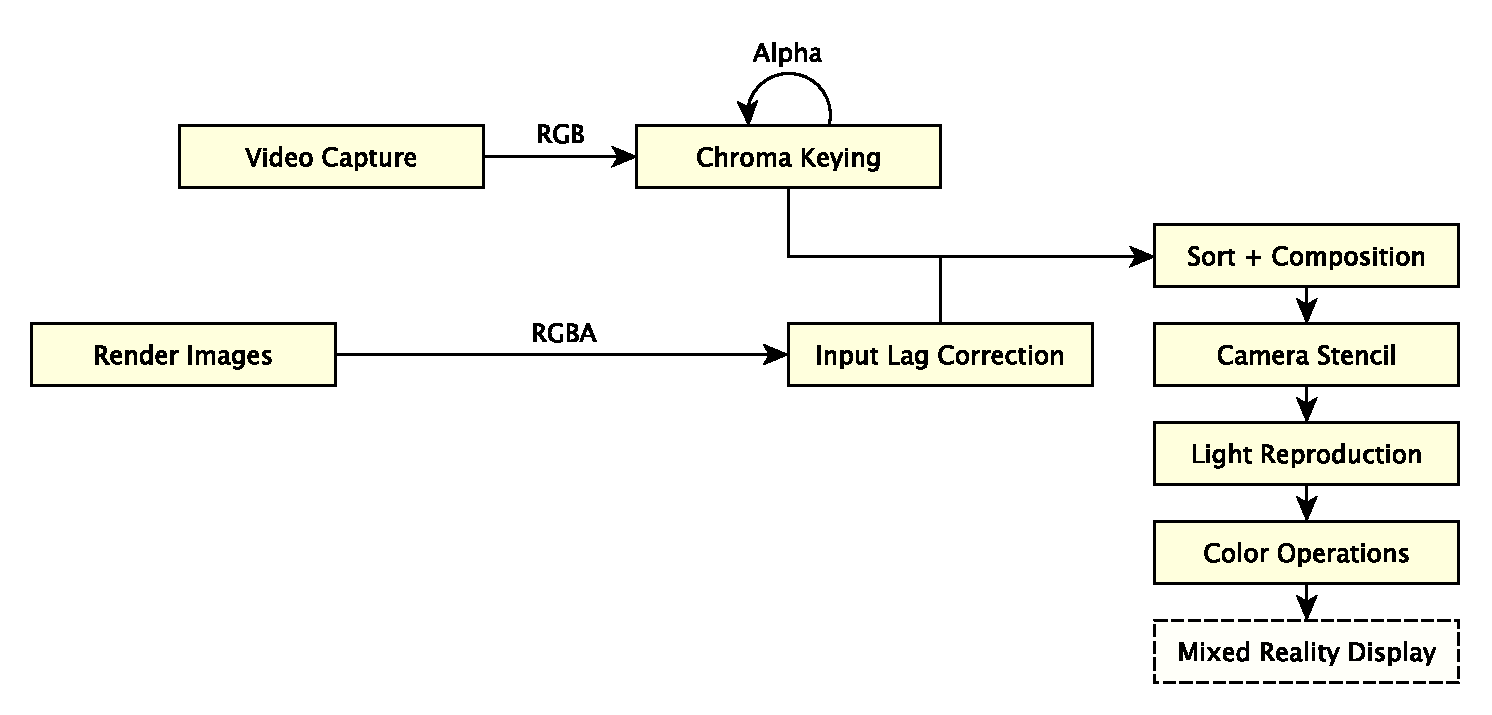
\includegraphics[width=\textwidth]{_raw_resources/pipeline_steps/4_0_pipeline.pdf}
	\caption{Full mixed reality graphics pipeline in order of graphical 
	fidelity impact}
	\label{fig:steps:pipeline}
\end{figure}

The following chapter describes the techniques used to transform motion video 
inside a green screen into a mixed reality image. As brief overview, the steps 
required are performed in order of biggest impact in graphical fidelity (Fig. 
\ref{fig:steps:pipeline}) for the composition of a real world motion video 
feed. This is different to the actual render order but gives a better 
understanding of the techniques used to achieve a mixed reality imagery. A 
closing remark with the order of calculation has been added at the end of the 
chapter.

% !TeX spellcheck = en_US
% !TEX root = ../thesis-example.tex
%
\section{Chroma Key}
\label{sec:chromakey}

Beginning from a real-world camera, the video signal travels through the 
Inogeni 4KUSB3 converter and is accessible with the systems API for webcams. 
(See figure \ref{fig:system-components})

\begin{figure}[htb]
	\centering
	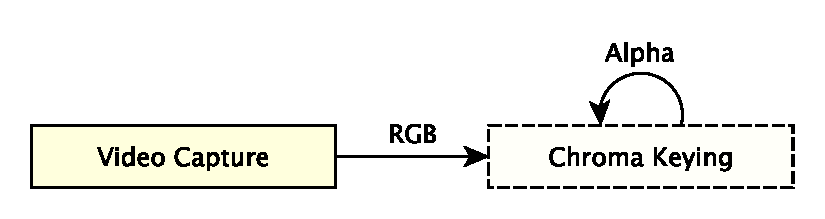
\includegraphics[width=.7\textwidth]{gfx/pipeline/4_1_chroma.pdf}
	\caption{Initial step upon receiving the camera image}
	\label{fig:steps:chroma}
\end{figure}

The initial step is to remove the green (or blue) background from the image, 
which should be live footage of a green (or blue) box. Other literature usually 
refers to it as "pulling a video matte" or "chroma keying." For a reference 
green, there has to be a color picked manually in the material editor of Unity 
--- this was made by a checkbox to show raw output from the camera (eg. fig. 
\ref{fig:chroma:editor}). Then an average green from the background box can be 
picked. This is an important setup step, since lightning situations can vary 
greatly and minor differences in light setups can have a great effect on the 
outcome of visible green background captured by the camera, thus making a 
recalibration necessary.

\begin{figure}[htb]
	\centering
	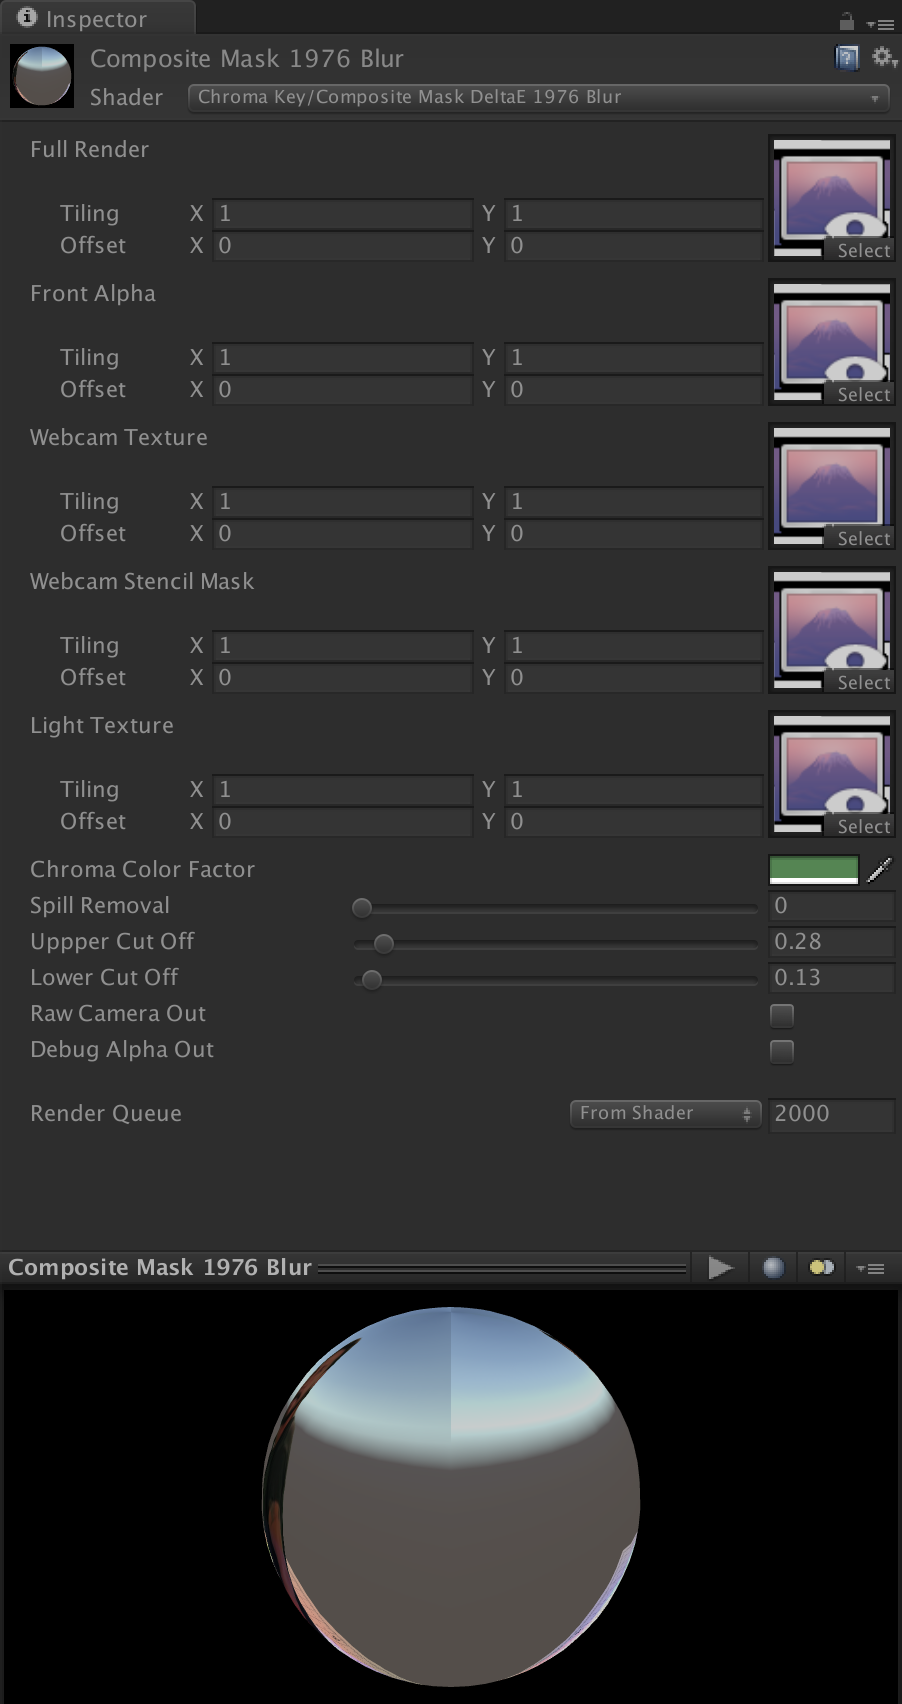
\includegraphics[width=.45\textwidth]{gfx/distances/material-editor.png}
	\caption{Material Editor inside Unity}
	\label{fig:chroma:editor}
\end{figure}

An extreme example case is used for comparing different chroma keying variants, 
which shows high motion blur due to a low shutter speed of the capturing 
camera and fast movement of the depicted actor:

\begin{figure}[htb]
	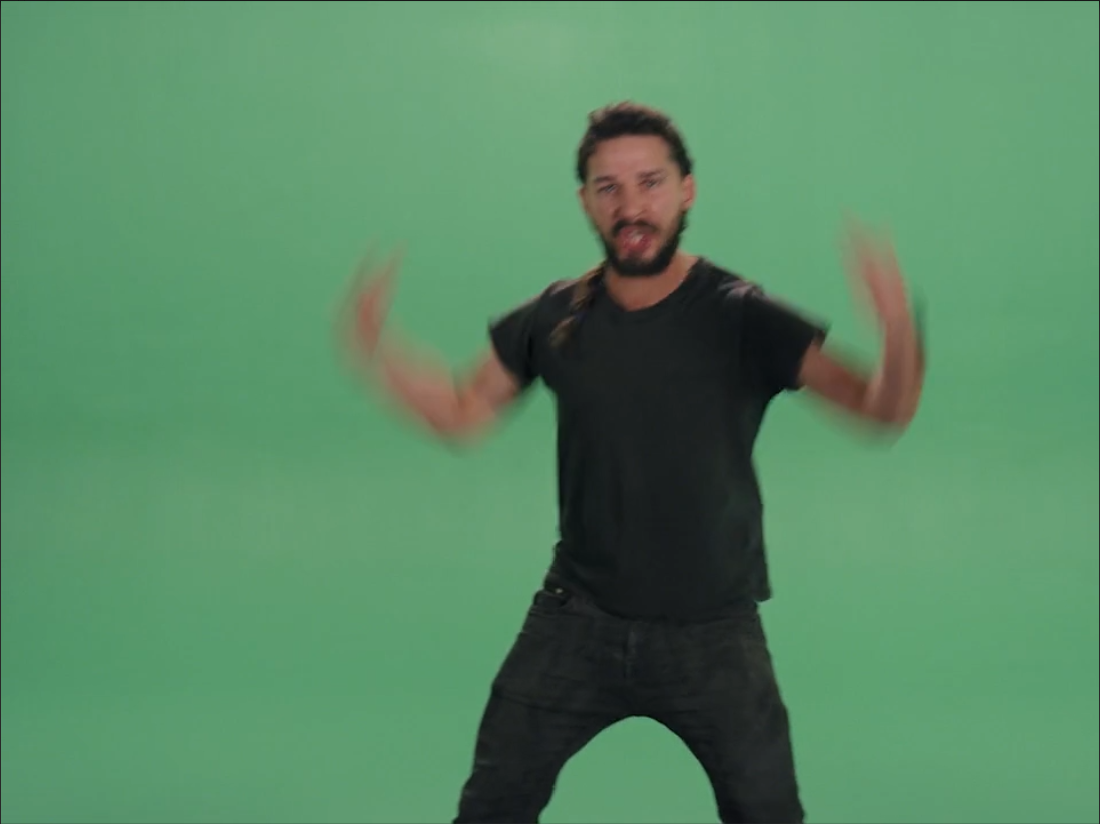
\includegraphics[width=\textwidth]{gfx/distances/example.png}
	\caption{Comparison Image \cite{vimeo:shia:2015} --- sRGB Output}
	\label{fig:chroma:color}
\end{figure}

\subsection{Initial Assumption}

Each RGB color can be represented as a discrete 3-Vector of (red, green and 
blue)  values in range of $[0, 1]$\footnote{Software RGBA color representations 
usually take 8bit per color channel and map between $[0, 255]$ --- graphic 
computing usually maps between $[0, 1]$}. An interpolation between two colors 
can be summarized as a matting equation as follows, where a foreground image 
$C_F$ and a background image $C_B - \alpha_B$ is assumed to be $1$:

\eq{eq:chroma:assumption:alpha:1}{
	I_{x, y} = \alpha_{x, y} C_{F_{x, y}} + (1 - \alpha_{x, y}) C_{B_{x, y}}
}

This matting equation has to be generalized for a later step, where 
$\protect\alpha$ is a value between [0, 1] on fore- and background, yielding a 
total Alpha of $\alpha_T$ as following:

\eq{eq:chroma:assumption:alpha:weak}{
	\alpha_T = \alpha_B * (1 - \alpha_F) \\
}

thus:

\eq{eq:chroma:assumption:alpha:cont}{
	I_{x, y} = (1 - \alpha_T) F_{x, y} + \alpha_T B{x, y}
}

This equation can take $\alpha_T < 1$ into account, which is needed later when 
fore- and background of the virtual environment are merged with a layer in 
between that results from the real world capture.

\subsection{Euclidean RGB Distance}
Assuming a source pixel color $C_S$ and a reference color $C_R$ we can 
calculate the euclidean distance between these two color vectors:
\eq{eq:euclidianrgb}{
	\alpha = \sqrt{(C_RR - C_SR)^2 + (C_RG - C_SG)^2 + (C_RB - C_SB)^2}
}

\begin{figure}[htb]
	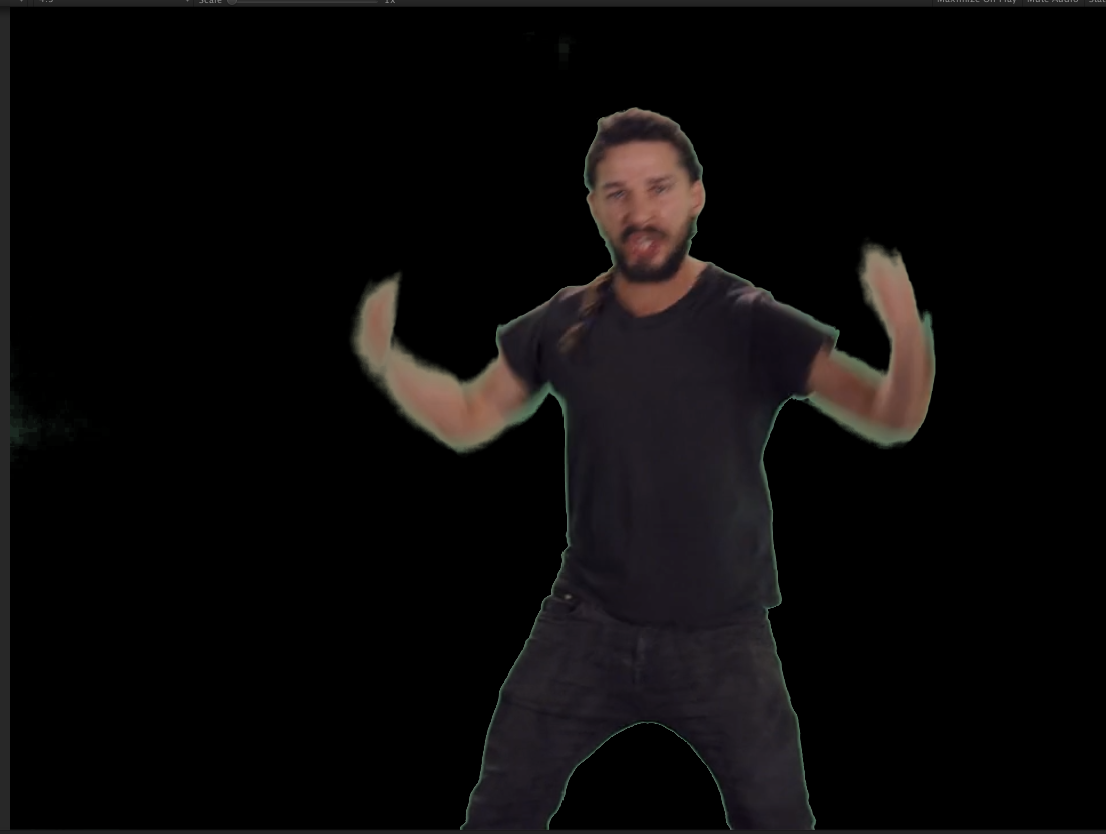
\includegraphics[width=\textwidth]{gfx/distances/chroma-rgb.png}
	\caption{Chroma Keying by using euclidean RGB distance}
	\label{fig:chroma:euclidean:rgb}
\end{figure}

This is computationally very low cost and works well enough to detect a 
difference between two distinct colors. It fails to accommodate for coloring 
that is perceived as different, but tinted by the reference colors. Since the 
green screen material will never achieve 0\% reflectivity, some color will 
spill onto the filmed actor and will therefore generate unwanted chroma-keying 
artifacts, most noticeable on semi-glossy reflection of skin or color tints on 
white clothing.

\subsection{Euclidean YCgCo Distance}

YCgCo gets its name for Luminance (Y), chrominance green (Cg) and chrominance 
orange (Co) and helps decorrelating color spaces by splitting color-lightness 
from color chrominances, thus splicing the color model into brightness and 
color appearance. Since it is a fast, lossless color transformation it 
is used in example for H.264 video encoding and other image compression 
techniques. The two chrominance channels are then split into green to magenta 
and orange to blue color channels and allow for a more accurate distance 
calculation between two colors.

\begin{figure}[htb]
	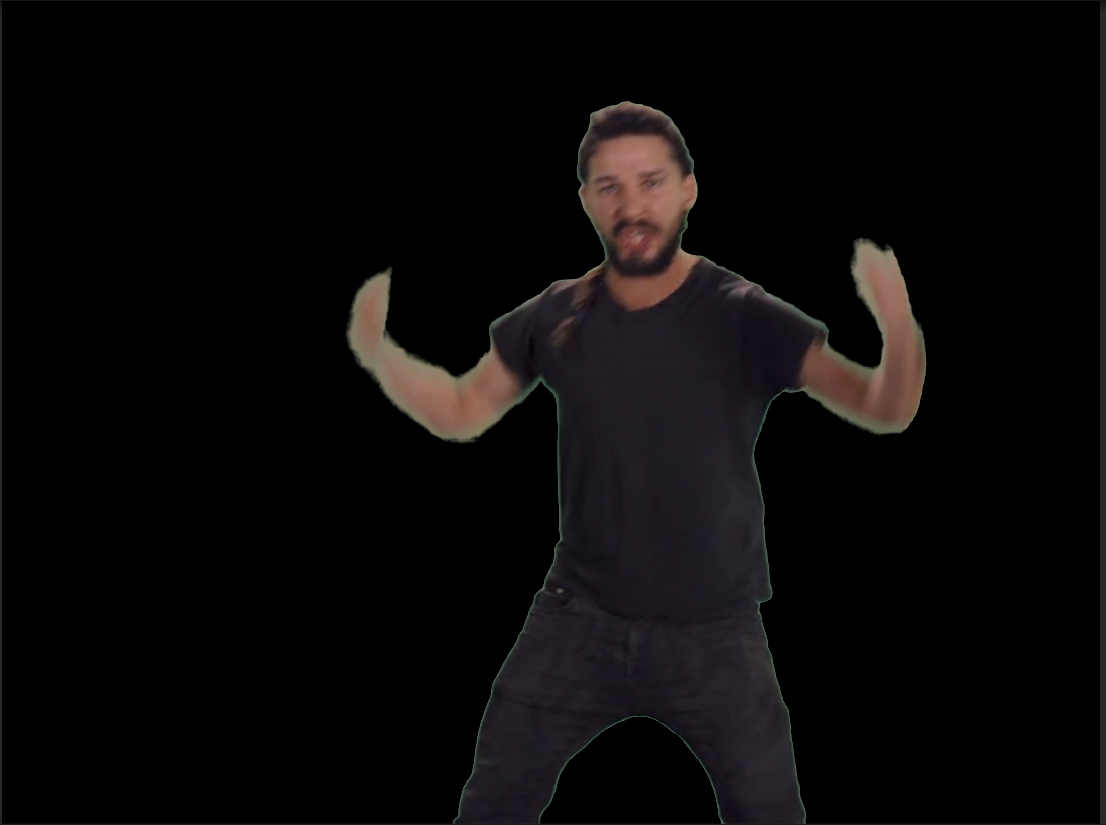
\includegraphics[width=\textwidth]{gfx/distances/chroma-ycgco.png}
	\caption{Chroma Keying by using euclidean YCgCo distance}
	\label{fig:chroma:euclidean:ycgco}
\end{figure}

Transforming any RGB color to YCgCo can be done with a single matrix  
multiplication, which is --- again --- a very low-cost computation on a GPU:

\eq{eq:ycgco:transformation}{
	\begin{bmatrix}
		Y \\
		Cg \\
		Co \\
	\end{bmatrix}
	=
	\begin{bmatrix}
		 \frac{1}{4} && \frac{1}{2} &&  \frac{1}{4} \\
		-\frac{1}{4} && \frac{1}{2} && -\frac{1}{4} \\
		 \frac{1}{2} && 0           && -\frac{1}{2}
	\end{bmatrix}
	*
	\begin{bmatrix}
		R \\
		G \\
		B 
	\end{bmatrix}
}

Given two colors, one from the video source $C_S$ and a reference color $C_R$ 
it is now possible to calculate the euclidean distance on the two chrominance 
channels:

\eq{eq:ycgco:euclidean}{
	\alpha = \sqrt{(C_RCg - C_SCg)^2 + (C_RCo - C_SCo)^2}
}

Due to the increased decorrelation, the result is more accurate and shows less 
artifacts on target pixels, allowing for better matte pulling, less 
green edges and a more continuous, smooth image of an actor.

\subsection{Euclidean Lab Difference}
The International Color Consortium (ICC) defined 1976 \textit{Lab $\Delta$E} as 
a standard model of calculating color differences inside the \textit{Lab} color 
vector volume. The final distance calculation is a linear euclidean scalar as 
with all other models, but accommodates for perceived color differences. It is 
a more expensive computation and needs code branches, which will evaluate all 
branches first by the GPU before using either code path.

A reference white has to be used to convert RGB to the Lab color model to 
accommodate for different RGB color spaces\footnote{which are usually only 
different on stored image material like photos or video}. Luckily the given 
webcam signal defaults to sRGB D65 and does not need a configurable reference 
matrix based on a given color model to handle different RGB color standards.

sRGB conversion needs to be converted to linear RGB while respecting light 
energy per color channel, rather than relative, perceived color brightness: 

\eq{chroma:inversecompanding}{
	v \in \{r, g, b\} \land V \in \{R, G, B\}
}

where: 

\eq{chroma:inverseRGBcompanding}{
	v = \\
	\begin{cases}
		\frac{V}{12.92}                 & \quad \text{if } V \leq 0.0405 \\
		(\frac{V + 0.055}{1.055})^{2.4} & \quad \text{otherwise}
	\end{cases}
}

from there an linear RGB color can be converted to XYZ by the following 
equation:

\eq{chroma:conversioncalc}{
	\begin{bmatrix}
		X\\
		Y\\
		Z\\
	\end{bmatrix}
		=
	\begin{bmatrix}
		M
	\end{bmatrix}
	\begin{bmatrix}
		R\\
		G\\
		B\\
	\end{bmatrix}
}

where:

\eq{chroma:rgbmatrix}{
	\begin{bmatrix}
		M
	\end{bmatrix}
		=
	\begin{bmatrix}
		R X_r && G X_g && B X_b \\
		R Y_r && G Y_g && B Y_b \\
		R Z_r && G Z_g && B Z_b
	\end{bmatrix}
}


\eq{chroma:xyzmatrix}{
		\begin{bmatrix}
		X\\
		Y\\
		Z\\
	\end{bmatrix}
	\begin{bmatrix}
		M
	\end{bmatrix}
	=
	\begin{pmatrix}
		X_r / Y_r && X_g / Y_g && X_b / Y_g \\
		1 && 1 && 1 \\
		\frac{1-X_r-Y_r}{Y_r} && \frac{1-X_g-Y_g}{Y_g} && \frac{1-X_b-Y_b}{Y_b}
	\end{pmatrix}
}

The needed $\begin{bmatrix}M\end{bmatrix}$ for RGB D65 is defined as:

\eq{chroma:sRGBD65}{
	\begin{bmatrix}
		0.4124564 && 0.3575761 && 0.1804375 \\
		0.2126729 && 0.7151522 && 0.0721750 \\
		0.0193339 && 0.1191920 && 0.9503041 \\
	\end{bmatrix}
}

Based on a reference white $U_r \in \{X_r, Y_r, Z_r\}$:

\eq{chroma:xyz2lab:defines}{
	U \in \{X, Y, Z\} \land W \in \{L, a, b\}
}

\eq{chroma:xyz2lab:epsilon}{
	\epsilon = 0.008856 \land \kappa = 903.3
}

where:

\eq{chroma:xyz2lab:ref}{
	w_r = \frac{U}{U_r}
}

\eq{chroma:xyz2lab:channel}{
	f(w) = \\
	\begin{cases}
		\sqrt[3]{w_r}      & \quad \text{if } U > \epsilon \\
		\frac{\kappa w_r + 16}{116} & \quad \text{otherwise}
	\end{cases}
}


\eq{chroma:xyz2lab:conversion}{
	\begin{bmatrix}
		L \\
		a \\
		b \\
	\end{bmatrix}
	=
	\begin{bmatrix}
		116 f_y - 16 \\
		500 (f_x - f_y) \\
		200 (f_y - f_z)
	\end{bmatrix}
}

With this conversion from sRGB to linear RGB to XYZ to Lab we can now calculate 
the euclidian linear distance between two colors $C_S$ and $C_R$, which already 
have been converted to Lab:

\eq{chroma:cie76:distance}{
	\Delta E = \sqrt{(C_R L - C_S L)^2 + (C_R a - C_S a)^2 + (C_R b - C_S b)^2}
}

The resulting values are rated by their perceptive difference (after Mkrzycki 
et. al. \cite{mokrzycki:2012}):

\begin{tabular}[htb]{l | l}
	0.0 \dots 0.5 & the difference is unnoticeable \\
	0.5 \dots 1.0 & the difference is only noticed by an experienced observer \\
	1.0 \dots 2.0 & the difference is also noticed by an unexperienced observer 
	\\
	2.0 \dots 4.0 & the difference is clearly noticeable \\
	4.0 \dots 5.0 & fundamental color difference  \\
	> 5.0 		  & gives the impression that these are two different 
	colors
\end{tabular}

Now it's possible to map alpha values for each pixel based on $\Delta$E 
distances between $m, n$ by clamping and biasing $\Delta$E with a proposed 
"smooth step" algorithm:

\eq{chroma:cie76:clamp}{
	f({\Delta E}) = x = \frac{\Delta E - n}{m - n}
}

\eq{chroma:cie76:min/max}{
	g(f({\Delta E})) = y =
	\begin{cases}
		n        & \quad \text{if } x \leq n \\
		x        & \quad \text{if } n \leq x \leq m \\
		m        & \quad \text{if } m \leq x
	\end{cases}
}

\eq{chroma:cie76:mapping}{
	\alpha(I_{x, y}) = 3 y ^2 - 2 y ^3
}

With that we receive a more natural matte with nearly no green edges, 
continuous actor imagery and smooth alpha transition between actor and green 
screen. Motion blur is hard to account for and is even with professional video 
matting hardware, extensive post production or intrinsic frame matting 
algorithms hard to remove without rough image results.

\begin{figure}[htb]
	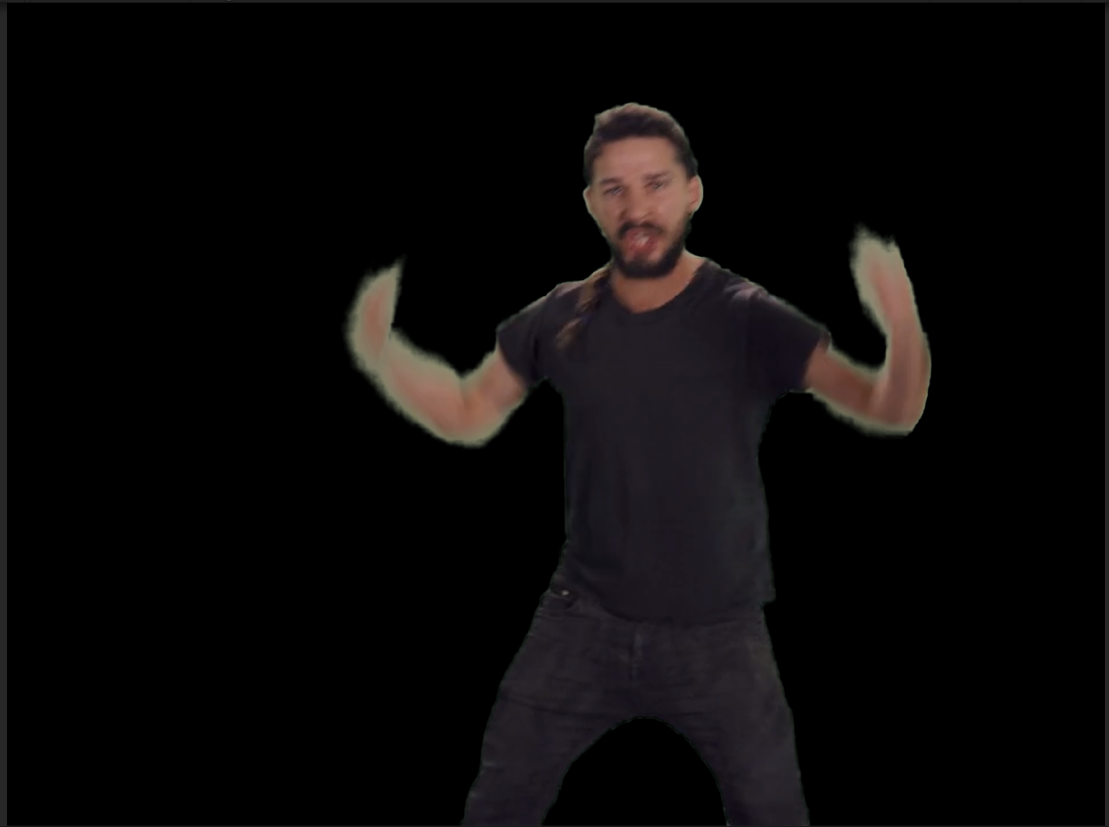
\includegraphics[width=\textwidth]{gfx/distances/chroma-deltae.png}
	\caption{Chroma Keying by using $\protect\Delta $E distance}
	\label{fig:chroma:deltae}
\end{figure}

\subsection{Comparison between Computational Models}

To chose the best variant, balancing runtime and efficiency, there has to be a 
comparison between the presented methods. Again, the previous image will be 
used, since it has complicated color mixing between background and actor. First 
we pick scan line of the image, in this case the 301st row from top, and 
calculate the color distance from each pixel to a reference color $[R, G, B] = 
[0.341, 0.588, 0.42]$.

As seen in figure \ref{fig:chroma:image_comparison}d, CIEDE76s performance is 
significantly better in separating colors and has a broader margin between 
green background and other foreground. This can be observed in figure 
\ref{fig:chroma:image_comparison}, where the scan line is set as background and 
the values are normalized again:

\begin{figure}[htbp]
	\caption{Comparison between different color distance methods}
	\label{fig:chroma:image_comparison}
	\begin{subfigure}[t]{.65\textwidth}
		\centering
		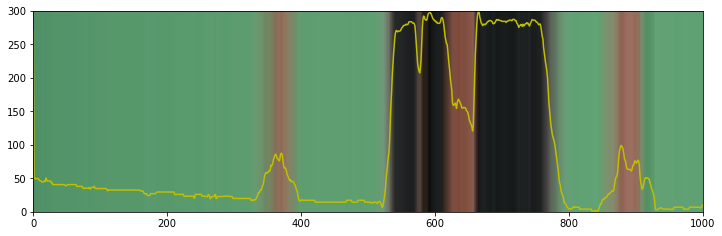
\includegraphics[width=\textwidth]{gfx/distances/color-rgb.png}
		\caption{RGB color distance} 
	\end{subfigure}
	\begin{subfigure}[t]{.3\textwidth}
		\centering
		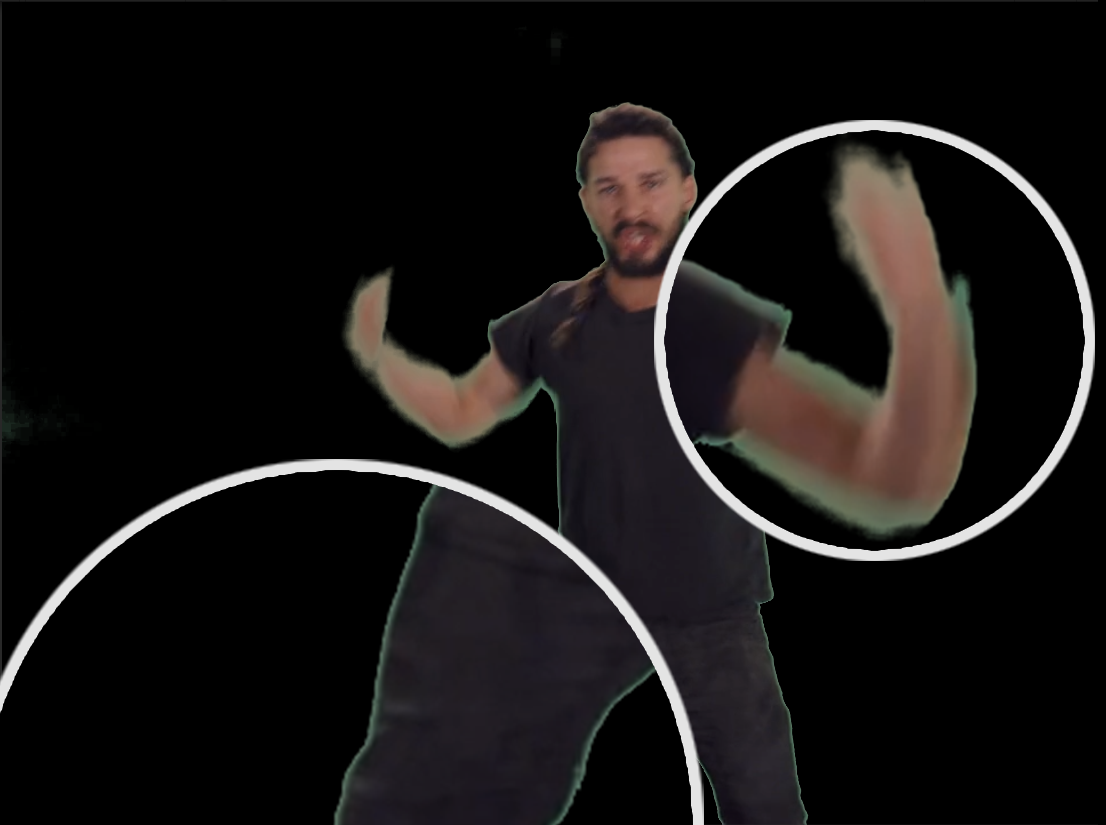
\includegraphics[width=\textwidth]{gfx/distances/zoom-rgb.png}
	\end{subfigure}
	\begin{subfigure}[t]{.65\textwidth}
		\centering
		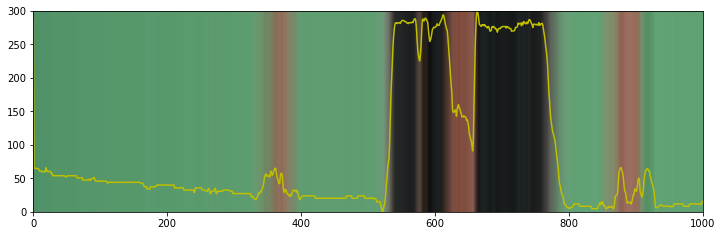
\includegraphics[width=\textwidth]{gfx/distances/color-ycgco.png}
		\caption{YCgCo color distance}
	\end{subfigure}
	\begin{subfigure}[t]{.3\textwidth}
		\centering
		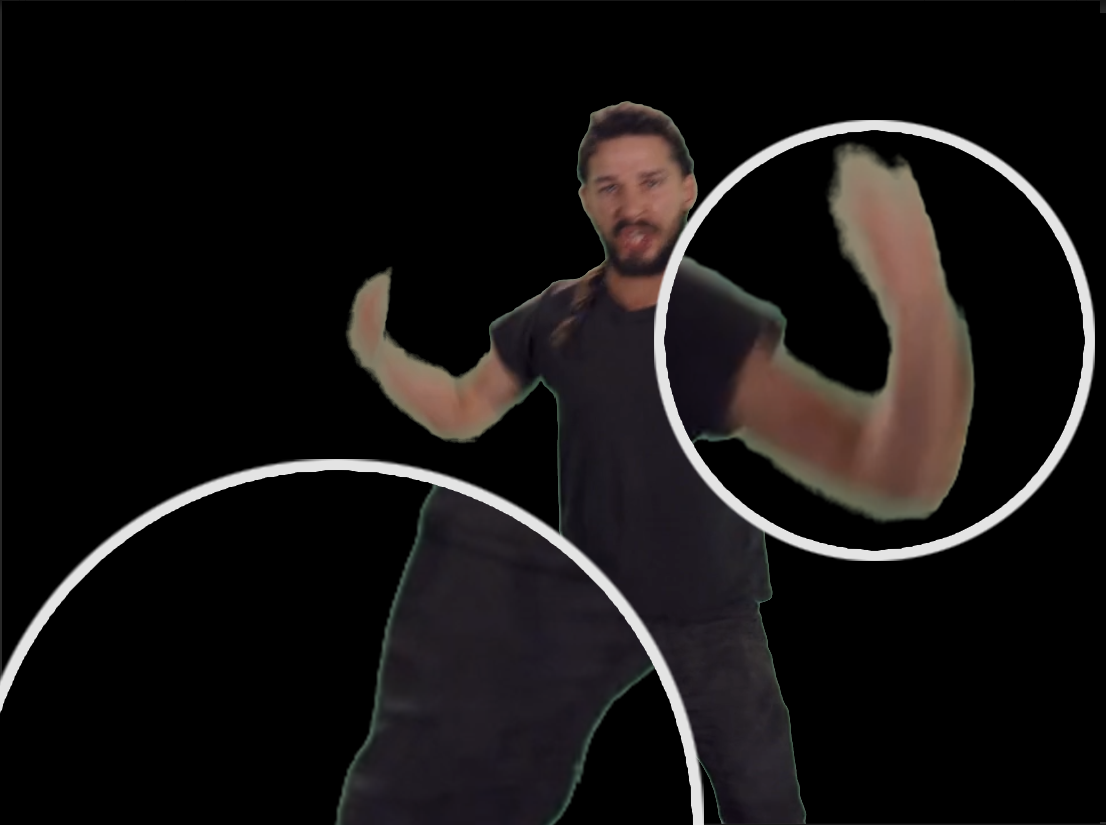
\includegraphics[width=\textwidth]{gfx/distances/zoom-ycgco.png}
	\end{subfigure}
	\begin{subfigure}[t]{.65\textwidth}
		\centering
		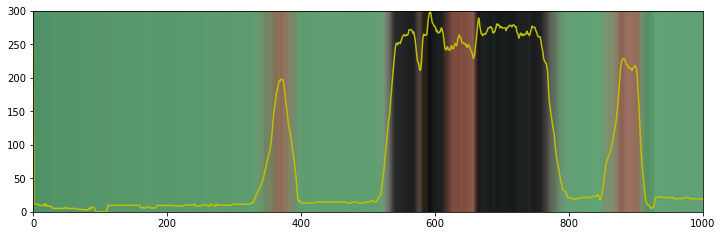
\includegraphics[width=\textwidth]{gfx/distances/color-ciede76.png}
		\caption{CIEDE76 color distance}
	\end{subfigure}
	\begin{subfigure}[t]{.3\textwidth}
		\centering
		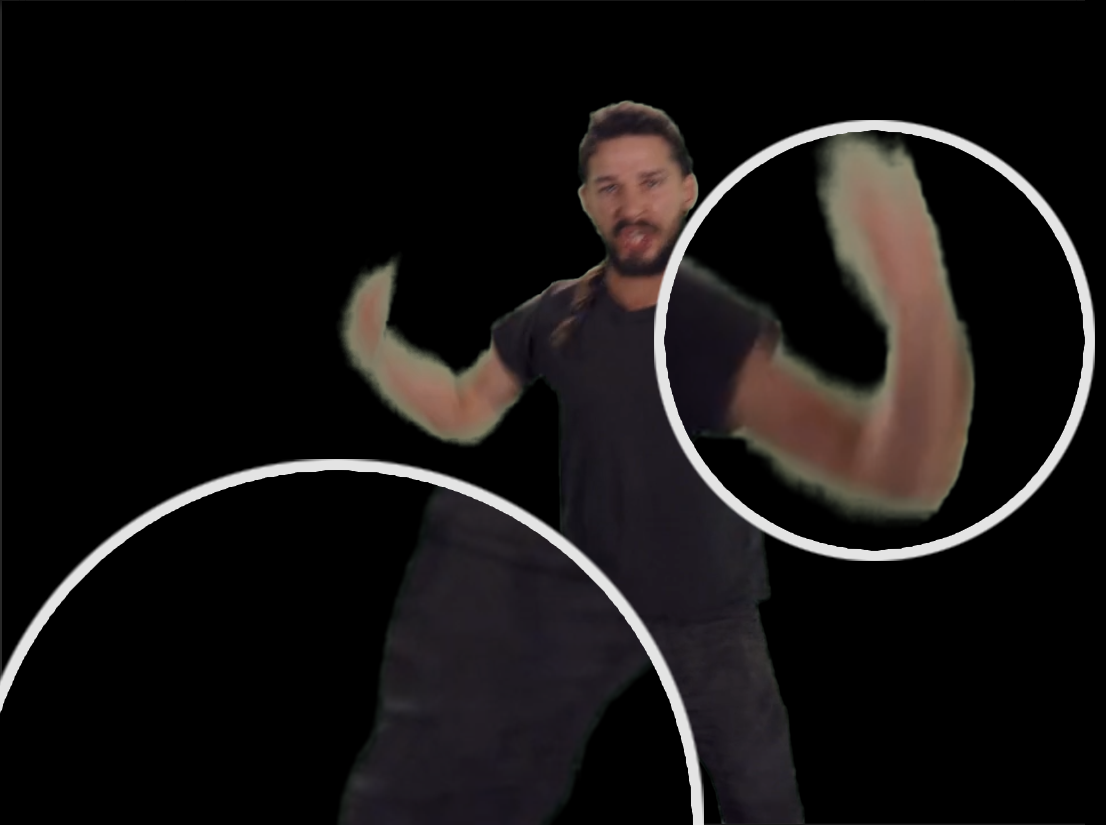
\includegraphics[width=\textwidth]{gfx/distances/zoom-delta_e.png}
	\end{subfigure}
	\begin{subfigure}[t]{\textwidth}
		\centering
		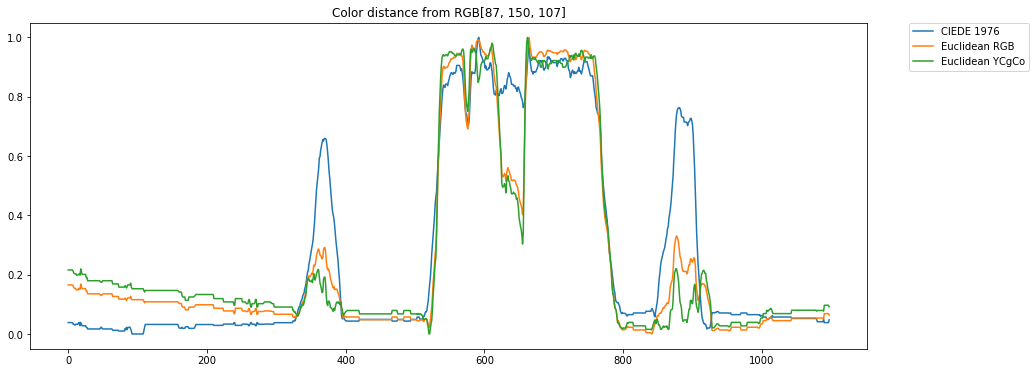
\includegraphics[width=\textwidth]{gfx/distances/dist-comp.png}
		\caption{Normalized graph comparing color difference methods}
	\end{subfigure}
	\begin{subfigure}[t]{\textwidth}
		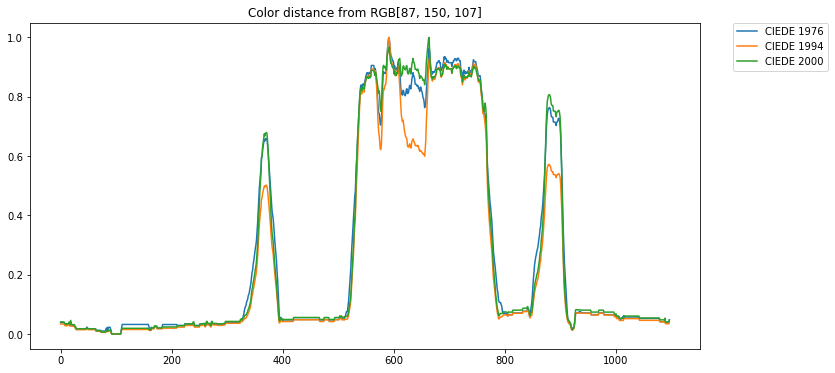
\includegraphics[width=\textwidth]{gfx/distances/ciede-comp.png}
		\caption{Comparison with different CIEDE $\Delta E$ variants}
	\end{subfigure}
\end{figure}
Additionally, CIEDE76 shows less variance on similar colored spaces to the 
target color as well as high color difference peaks on all other pixels. This 
yields an accurate upper and lower limit, in which the green screen can be 
calibrated in.
\newline
Finally, comparing CIEDE76, CIEDE94 and CIEDE2000 reveals, that CIEDE76 
performs well enough while having the lowest performance overhead. The 
similarities between the 1976 and 2000 method are very apparent, while 
CIEDE2000 has a significantly more complex algorithm. (cf.  
\cite{sharma:ciede2000:2005}) Performing the same operation on the same data 
with different CIEDE color distance revisions (fig. 
\ref{fig:chroma:image_comparison}e), that there is little difference between 
CIEDE76 and CIEDE2000.        % Chroma Key Section
\section{Camera Offsets}

\begin{lstlisting}
	> Is this text?
	< No, this is doge.
\end{lstlisting}      % Render Buffer Swapper
% !TeX spellcheck = en_US
% !TEX root = ../thesis-example.tex
%
\section{Mitigating Frame Jitter}

An additional step that can be handled by the same algorithm is the mitigation 
of frame or time jittering, a term that describes a effect of different running 
framerates of an actors captured video footage and rate of 3D environment 
rendering. Since the native framerate of the HMD is higher than the frames 
produced by the video feed, there will be noticeable small jitters of virtual 
camera movement, which are not present on the source video material. The HTC 
Vive Controller are very good at picking up minuscule changes in motion, which 
are instantly translated to the transform of the camera rig and then result in 
minor motion of the 3D environment. Visually this shows in a shaking virtual 
world while the real world video stands still.
\newline
To minimize the effect, it is possible to overwrite framebuffers for as long as 
one duration of a video frame and then swapping out these buffers. The headset 
recommends to run it at 90fps - miss timings are no issue either, since it 
results in non noticeable errors in virtual projections while the displayed 
frame is stable visual performance is unaffected. Thus it is possible to write 
less than three times into a framebuffer, which is mitigated again by 
displaying the final result later - the final image is therefore unaffected 
besides imperceptible differences between the real world camera and its virtual 
position.

\todo[inline]{needs then lstlisting when the code further up is modified}
			  % Frame Jitter Mitigation
% !TeX spellcheck = en_US
% !TEX root = ../thesis-example.tex
%
\section{Virtual projection parameters from real world camera}
\label{sec:projection-params}
To produce a virtual projection there are four unknowns to solve for:

\begin{my_list}
	\item Position of the real world camera
	\item Rotation of the real world camera
	\item Field of View (FoV) of the camera
	\item Distance between the HMD and the real world camera
\end{my_list}

Luckily the former two are solved by the tracking solution, thus can be used 
directly as transformation matrix for the virtual camera - ignoring an 
additional offset from the actual controller to the camera, which is accounted 
for inside the software.
\newline
The calculation of a corresponding distance between a camera and the Vive HMD 
to control the virtual projection parameters can be solved, too: Since both 
devices are tracked, one natively and the other with a controller as 
tracking anchor, it can be calculated with the same euclidean distance as 
discussed earlier, with $C$ as camera position and $H$ as HMD position:

\eq{eq:zsort:distance}{
	Z = \sqrt{(C_X + H_X)^2 + (C_Y + H_Y)^2 + (C_Z + H_Z)^2}
}

\begin{figure}[htb]
	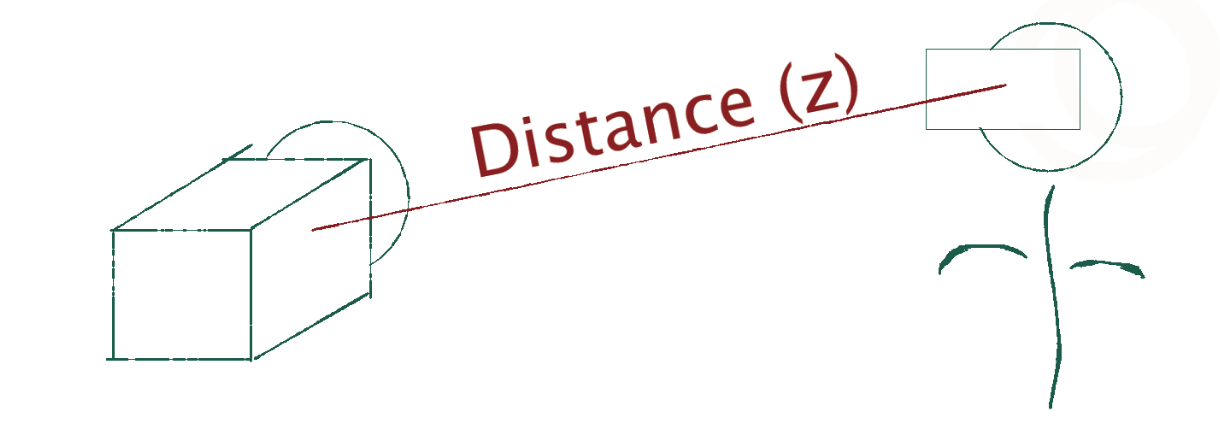
\includegraphics[width=\textwidth]{_raw_resources/composition/Composition-Z-Distance.png}
	\caption{Distance correlation}
	\label{fig:projection:distance}
\end{figure}

Another important projection parameter is field of view. Most production 
cameras only declare a focal length on lenses - which makes sense in that 
context, since field of view is a constraint between sensor size and focal 
length. Through the specification sheet of the camera the current field of view 
can be calculated inside Unity, with the sensor height as $S_h = 17.3mm$ and 
focal length as $F_l = 14mm$:

\eq{eq:zsort:fov}{
	FoV = 2*tan^{-1}\frac{S_h}{2 * F_l}
}

\eq{eq:zsort:fov:result}{
	FoV = 63.42028^\circ
}

With that we have now all projection parameters for the virtual environment to 
generate an image that matches in relative transformation parameters as the 
real world camera would look at. % Projection Parameters
% !TEX root = ../thesis-example.tex
%
\section{Virtual Z Sorting}

\todo[inline]{here a recap image of current steps: keying + delaying}

We have now a properly keyed video feed and synchronous motion between the VR 
actor and the 3D environment. To increase the immersion of that composition the 
next important step is to sort the scene on a tri-graph of planes.

\begin{figure}[htb]
	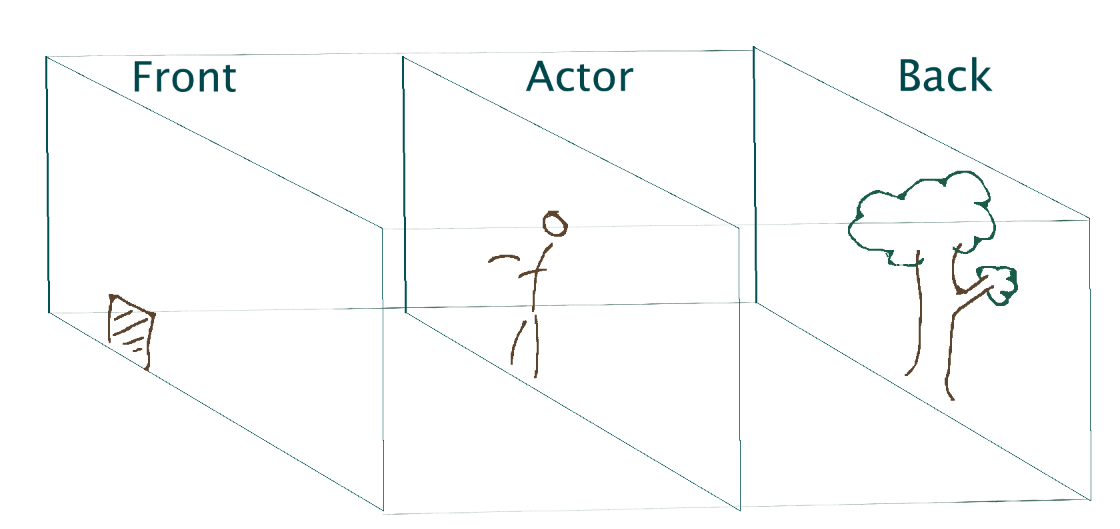
\includegraphics[width=\textwidth]{_raw_resources/composition/Composition-TriGraph.png}
	\caption{A sketch of the video composition with three layers of projection}
	\label{fig:zsort:sketch}
\end{figure}

There are multiple ways to achieve proper segmentation and composition of all 
three layers, depending on the rendering method. Deferred shading allows for 
better lightning simulation in engine but changes alpha- and depthmaps of a 
rendered scenery - this yields incorrect layer blending and results into an 
incorrectly displayed image. This software takes account for this and lets 
creators decide between two render modes:

\begin{my_list}
	\item Replace Masking: A front plane is displayed, after it follow the 
	chroma-keyed video and then the background. This is the most accurate image 
	generation.
	\item Alpha Masking: A front alpha mask of the geometry is displayed, then 
	the actor is mixed with a full render image of the background. The 
	resulting image has inconsistencies with alpha-blending but this method 
	works with all rendering setups.
\end{my_list}

The decision is between accuracy and presentation. Many post processing effects 
or deferred shading are not able - or simply do not respect - the alpha matte, 
which is usually no issue, since these steps are taken after rendering is 
complete, thus causing no unwanted side-effects. Other post effects need 
certain projection requirements and / or get disregarded through culling, like 
in Figure \ref{fig:zsort:comparison:front} where the volumetric lightning is 
culled out of the virtual projection and therefore gets completely ignored, 
resulting in a black front geometry.

\begin{figure}[htbp]
	\caption{A comparison of different composition methods in engine}
	\label{fig:zsort:comparison}
	\begin{subfigure}[t]{.45\textwidth}
		\centering
		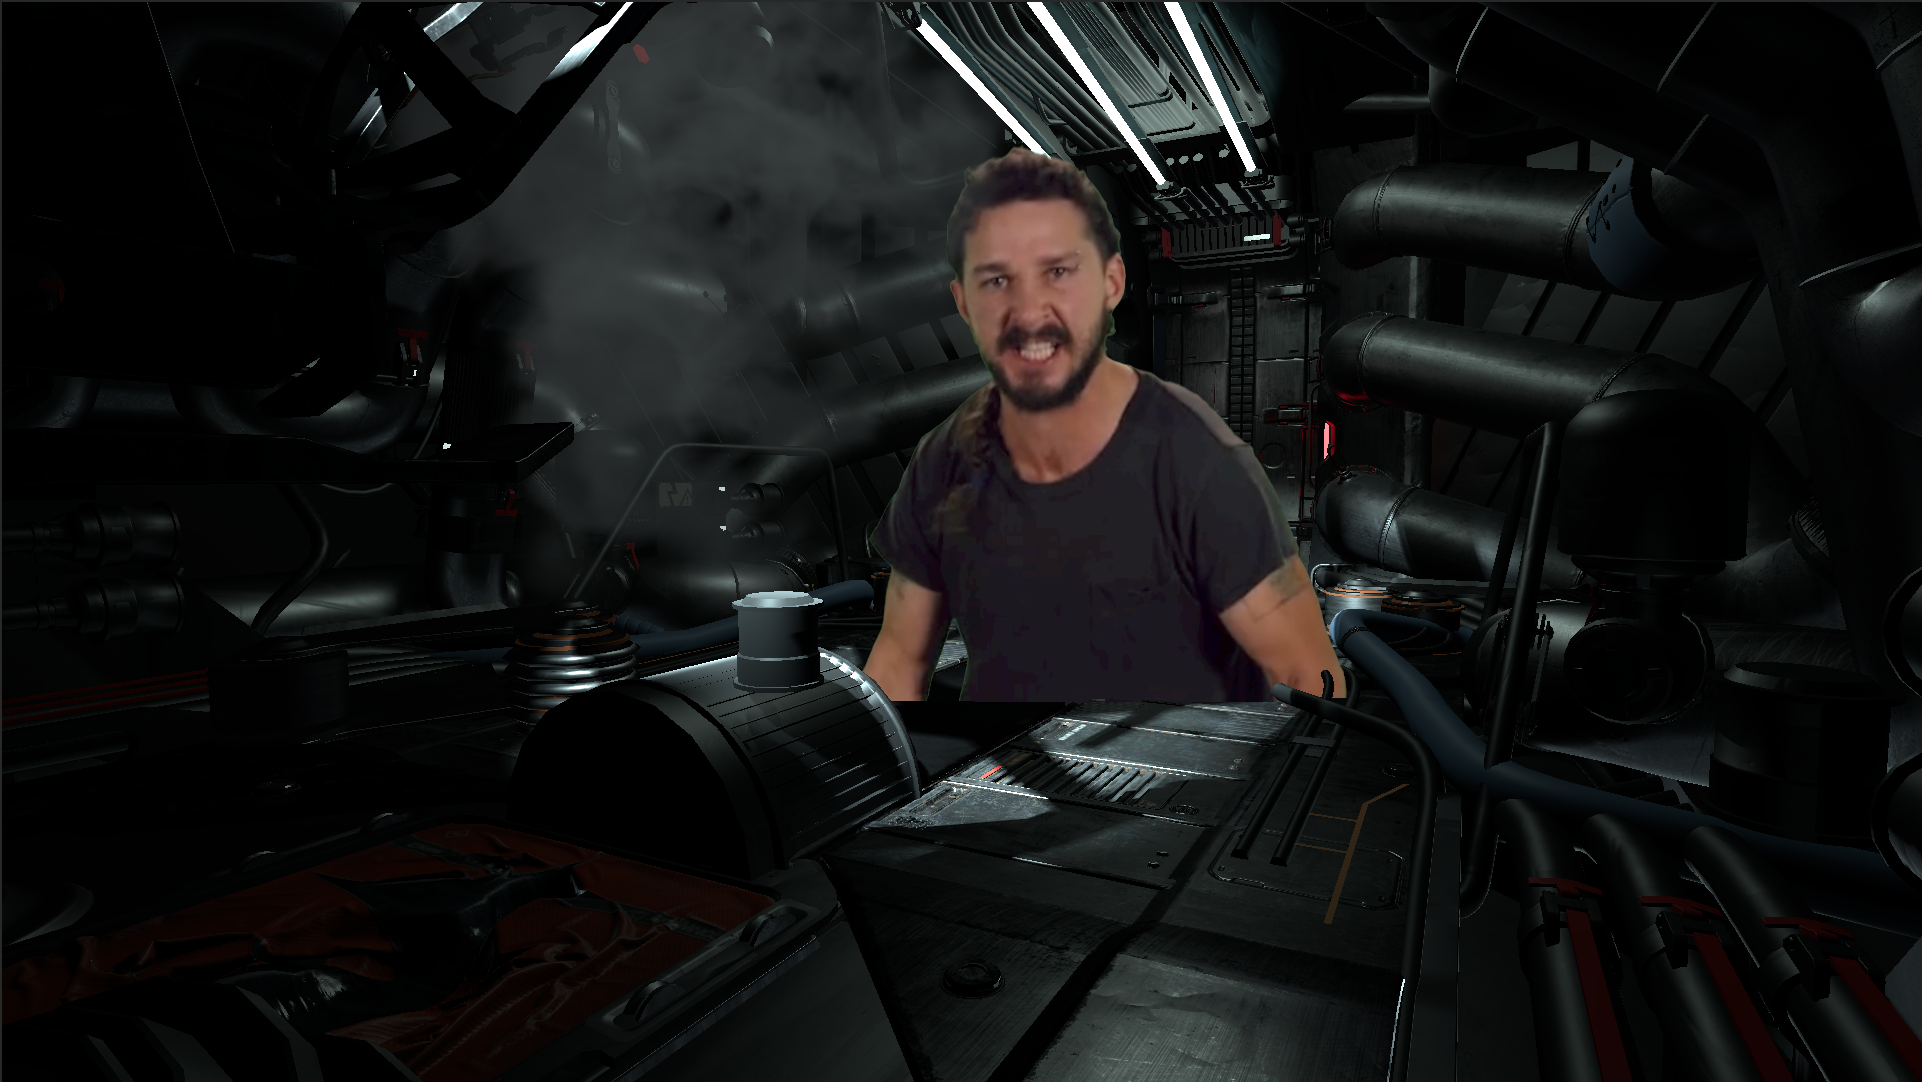
\includegraphics[width=\textwidth]{_raw_resources/composition/Composition-Perfect-Realigned.png}
		\caption{The proposed composition, simulated, with an arbitrary depth 
		of the video feed}
	\end{subfigure}
	\begin{subfigure}[t]{.45\textwidth}
		\centering
		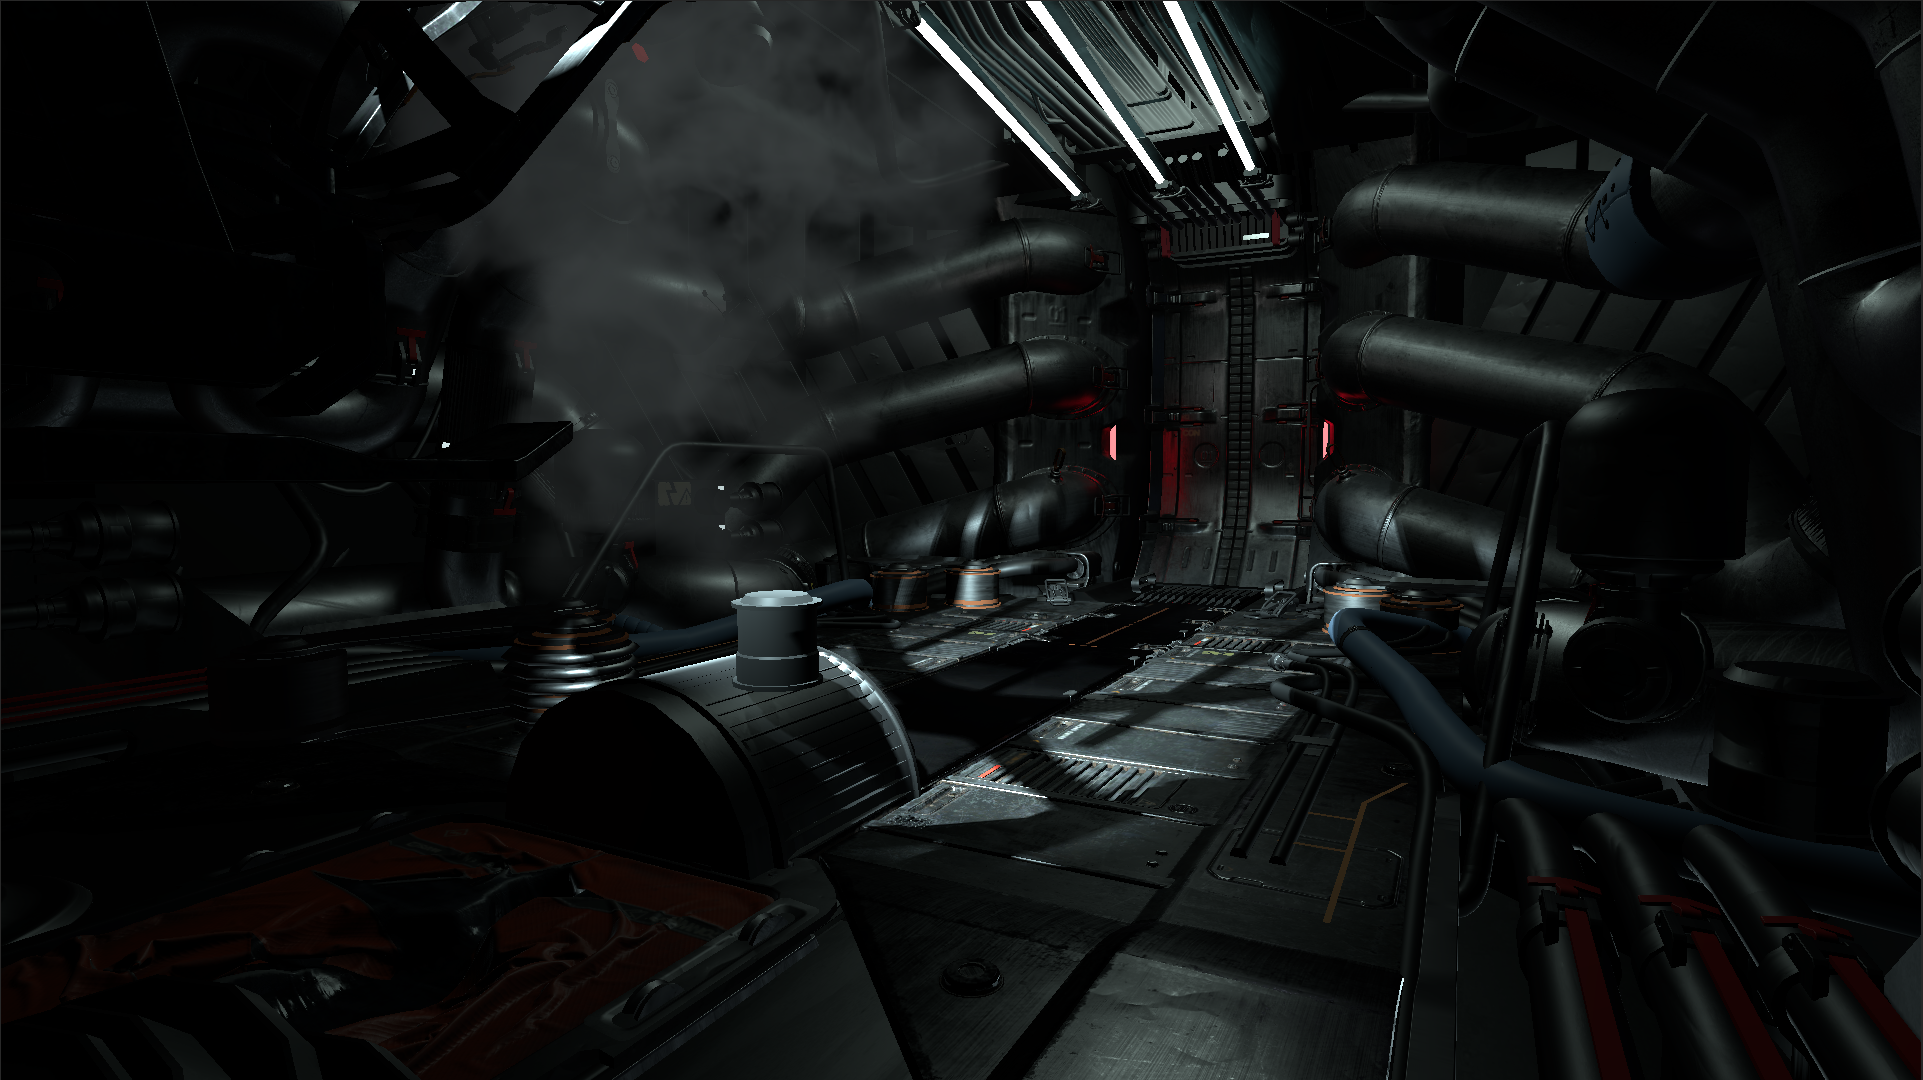
\includegraphics[width=\textwidth]{_raw_resources/composition/Composition-Full-Render.png}
		\caption{The full length rendering}
	\end{subfigure}
	\newline
	\begin{subfigure}[t]{.45\textwidth}
		\centering
		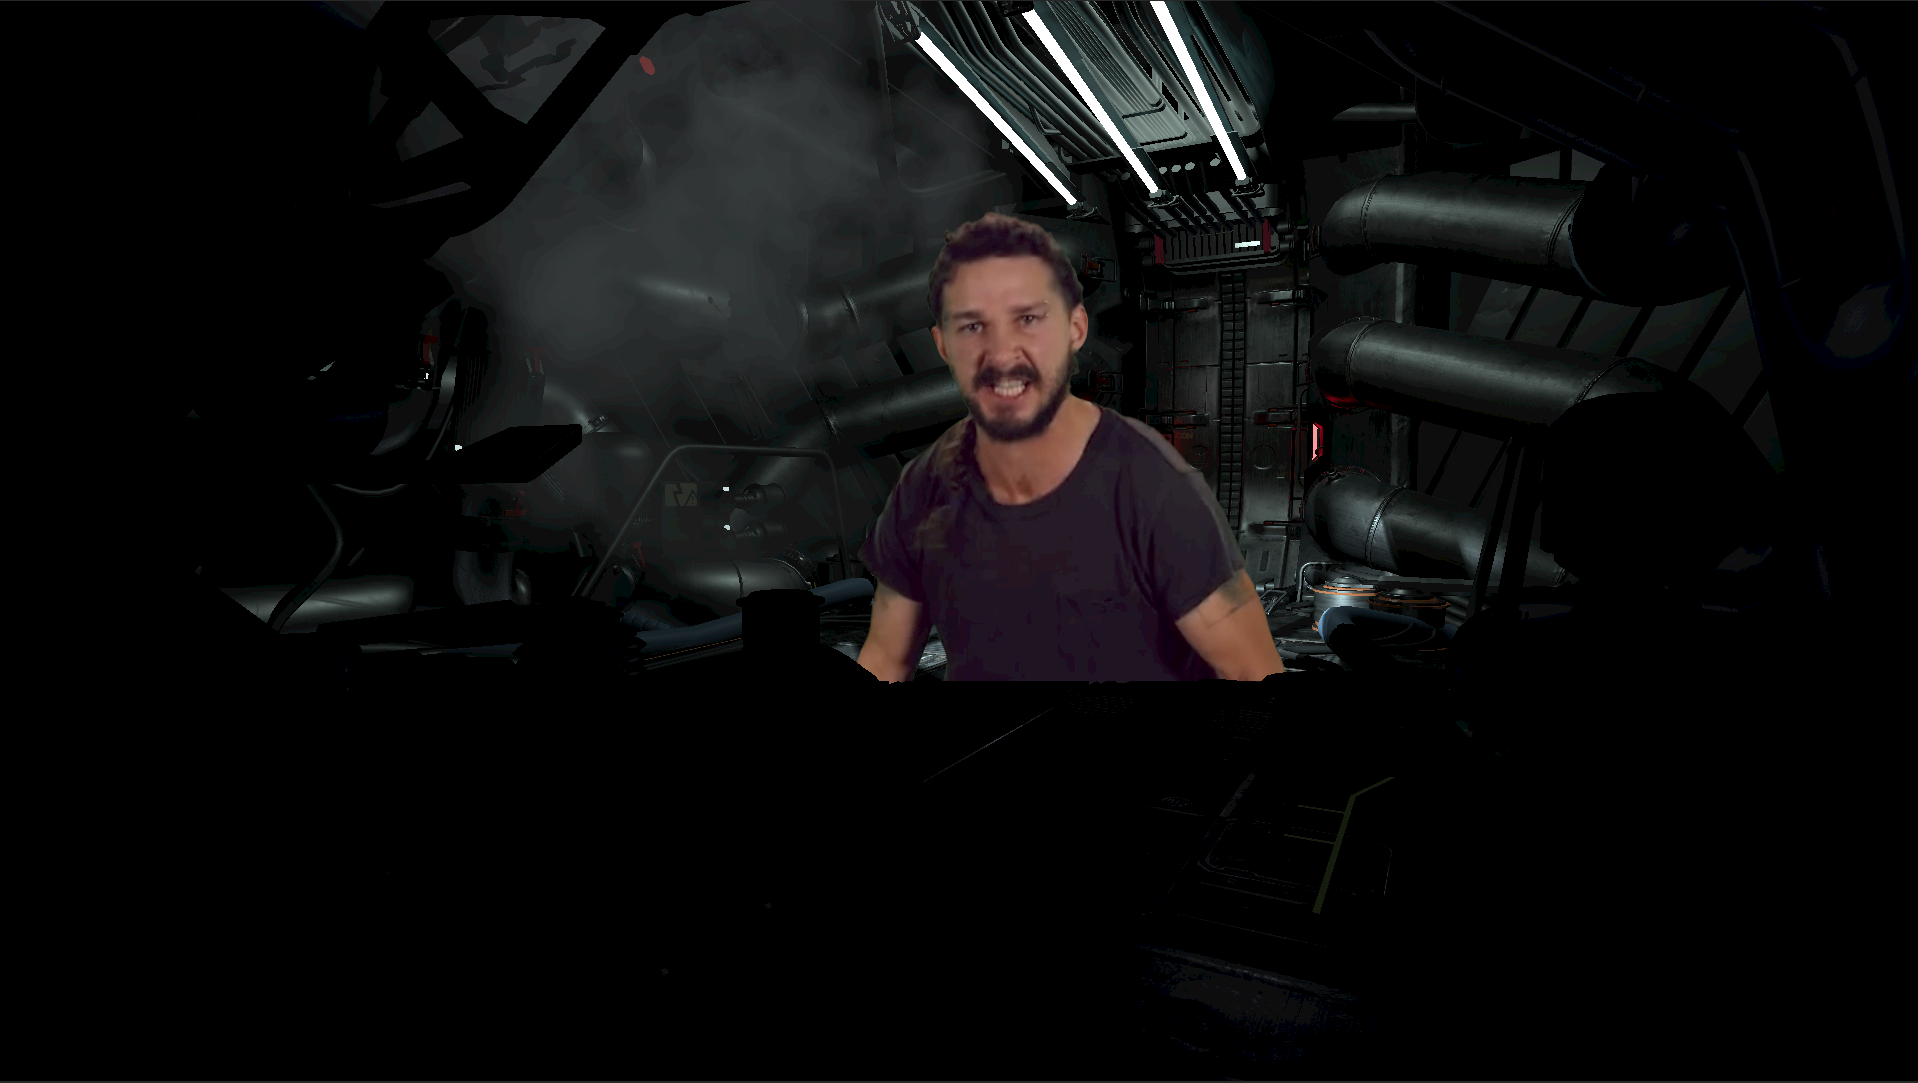
\includegraphics[width=\textwidth]{_raw_resources/composition/Composition-Front-Replace_orso.png}
		\caption{A composition by rendering a front, followed by the video and 
		then the background}
	\end{subfigure}
	\begin{subfigure}[t]{.45\textwidth}
		\centering
		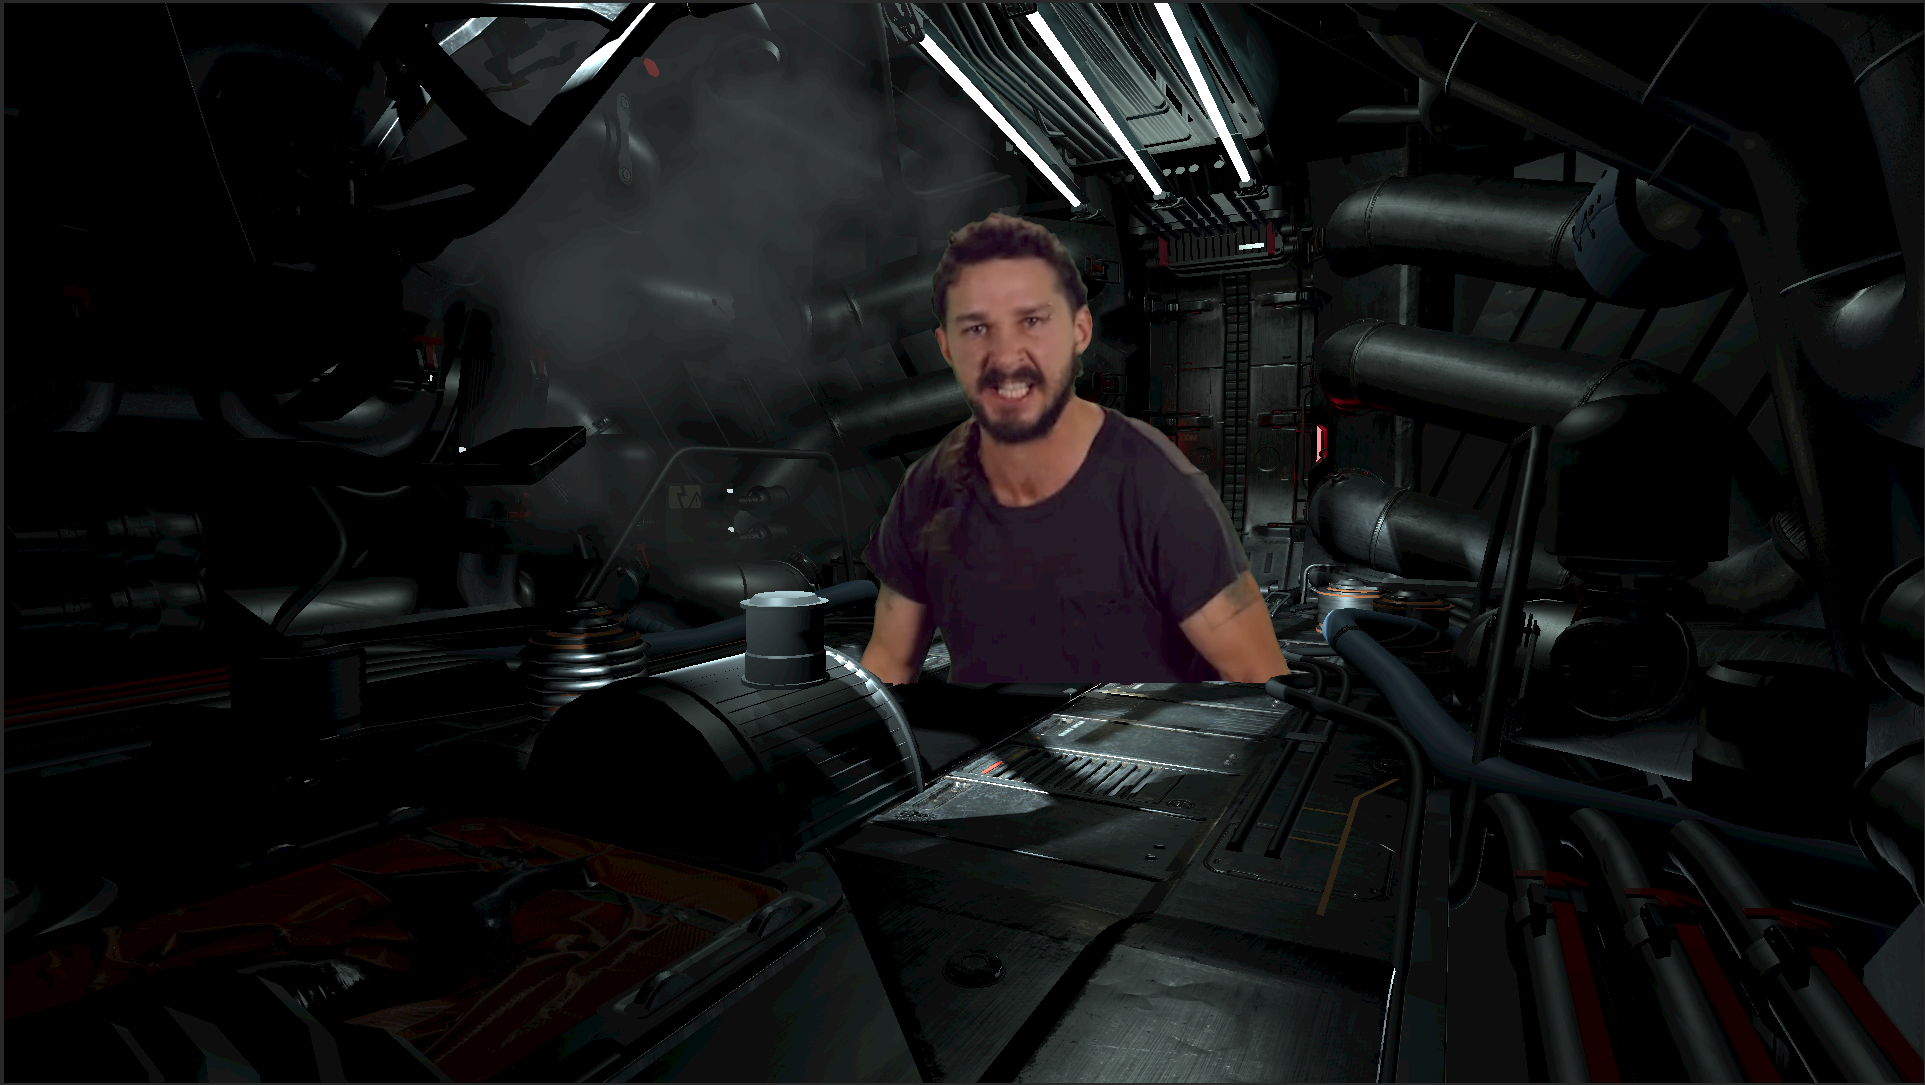
\includegraphics[width=\textwidth]{_raw_resources/composition/Composition-Front-Mask.png}
		\caption{A composition with the front geometry as mask, and then a 
		mixing of the video and a full length render}
	\end{subfigure}
	\newline
	\begin{subfigure}[t]{.45\textwidth}
		\centering
		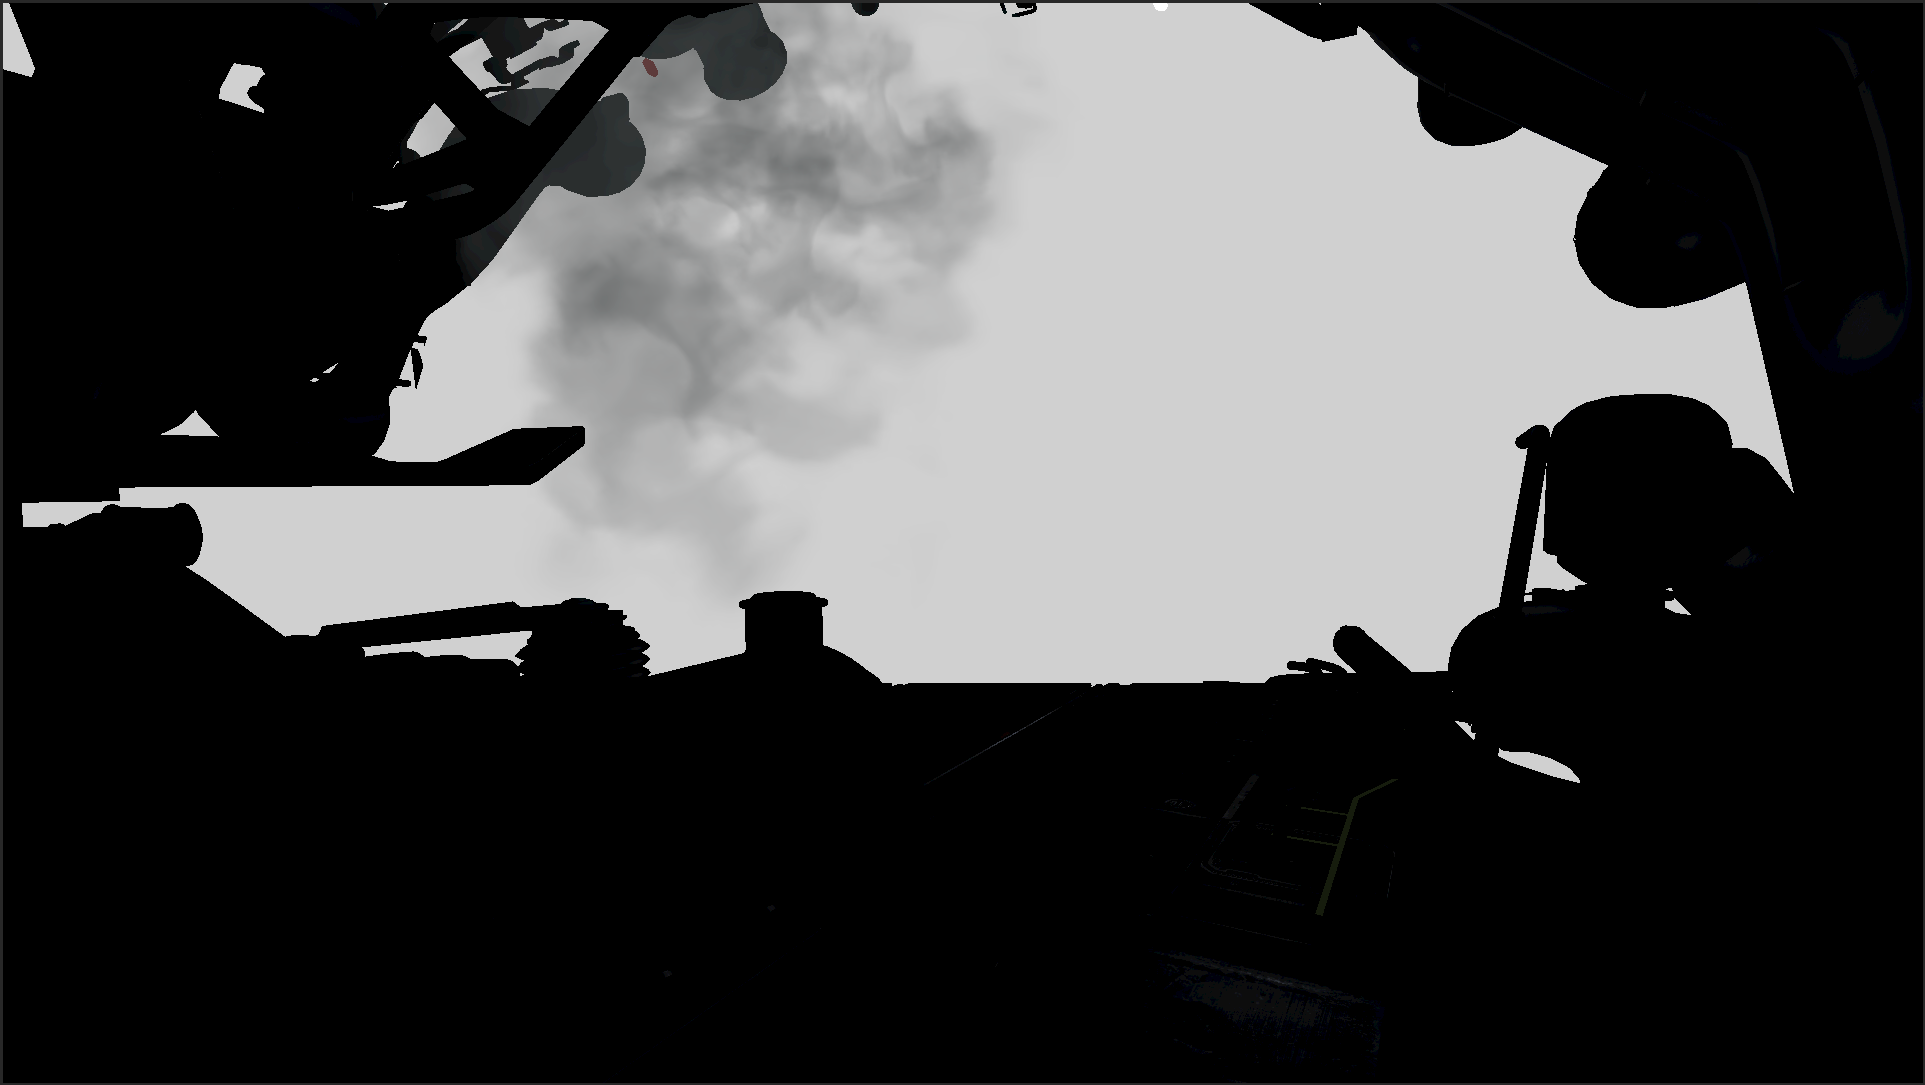
\includegraphics[width=\textwidth]{_raw_resources/composition/Composition-Front.png}
		\caption{The virtual projection of the front camera - volumetric 
		lightning does not work due to the short projection length}
		\label{fig:zsort:comparison:front}
	\end{subfigure}
	\begin{subfigure}[t]{.45\textwidth}
		\centering
		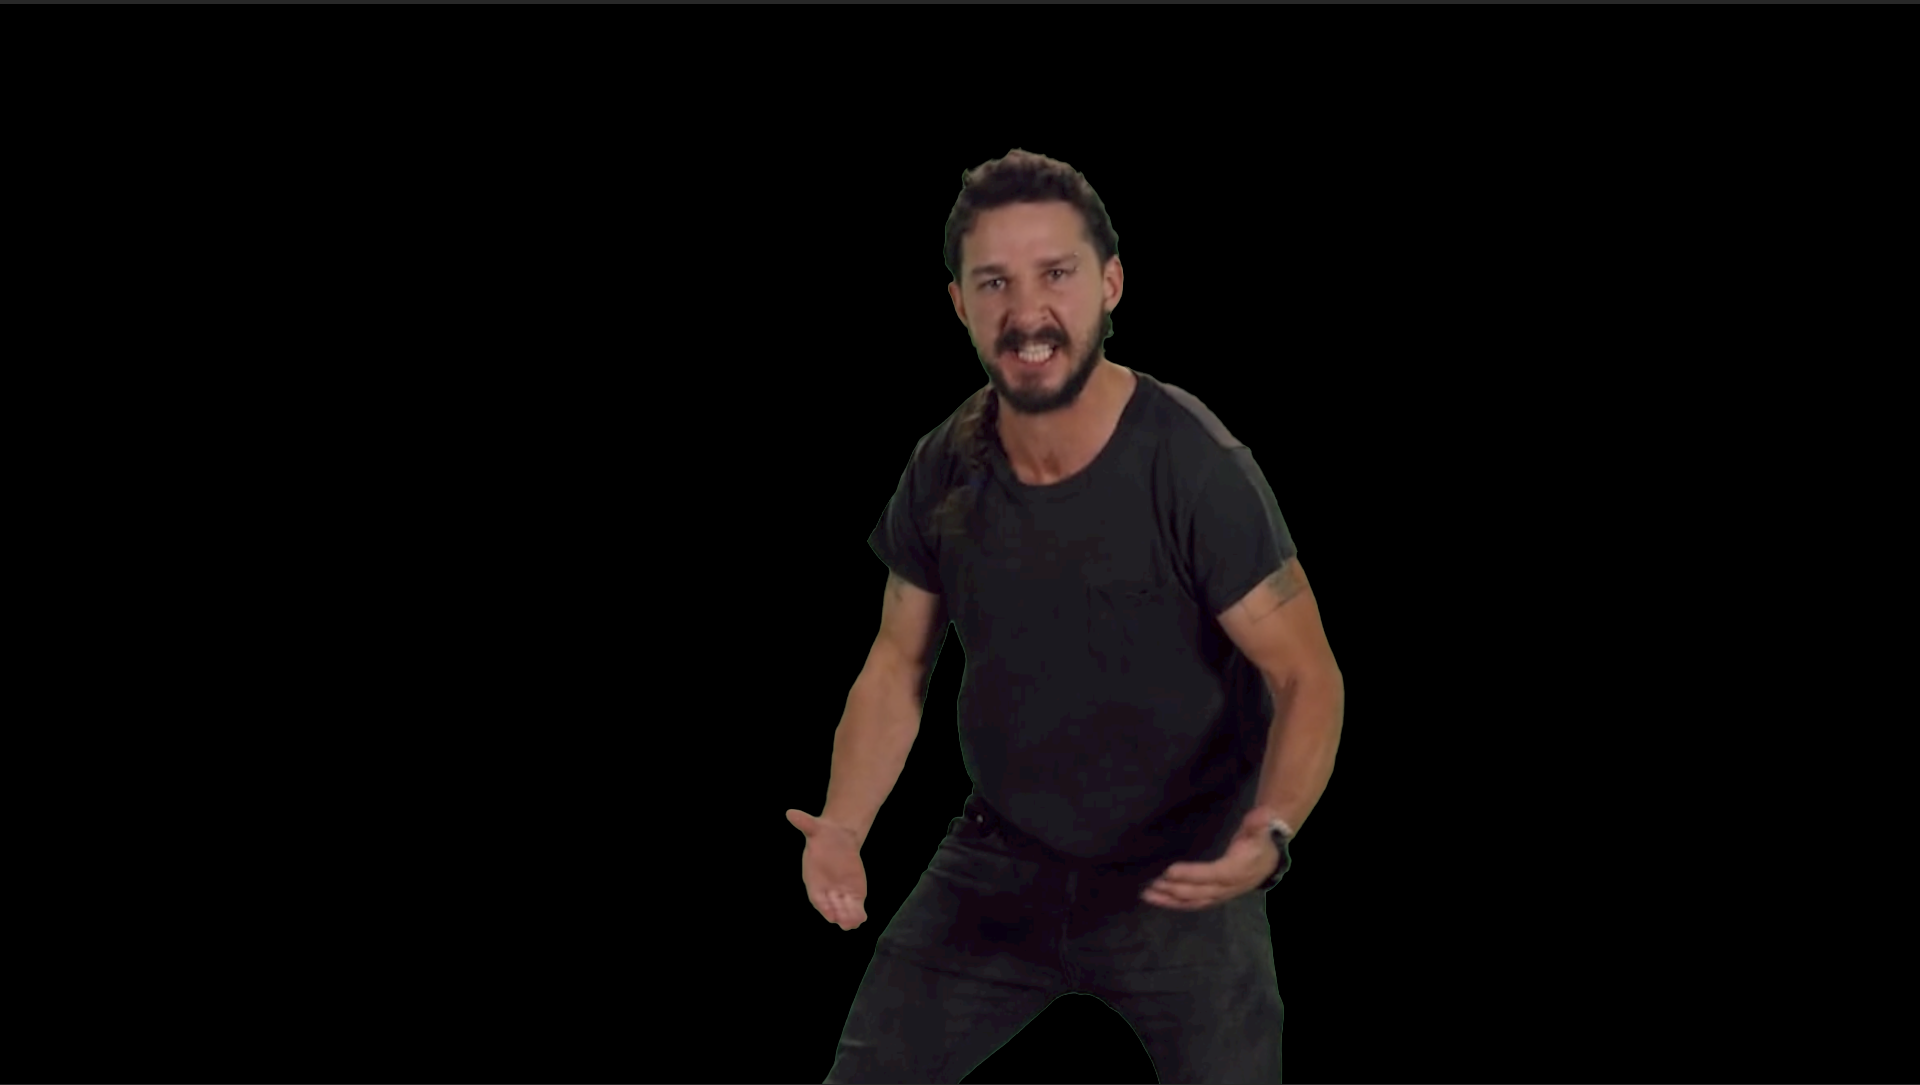
\includegraphics[width=\textwidth]{_raw_resources/composition/Composition-Chroma-Result.png}
		\caption{The chroma keying result}
	\end{subfigure}
\end{figure}

Mixing these three layers are similarly easy, using a previous equation 
\eqref{eq:chroma:assumption:alpha:weak} and 
\eqref{eq:chroma:assumption:alpha:cont}. Assuming an ARGB front render image 
$F$, a RGB video feed  $V$ and the RGB background $B$, 
we can mix all three layers effortlessly:

Replace Masking:

\eq{eq:zsort:replmask:1}{
	\alpha_T = \alpha_V * (1 - \alpha_F)
}


\eq{eq:zsort:replmask:2}{
	I(x, y) = (1 - \alpha_T) * F(x, y) + \alpha_T * V(x, y)
}

\eq{eq:zsort:replmask:3}{
	\alpha_S = \alpha_B * (1 - \alpha_{I(x, y)})
}


\eq{eq:zsort:replmask:4}{
	J(x, y) = (1 - \alpha_S) * I(x, y) + \alpha_S * B(x, y)
}

Alpha Masking is very similar with transforming the alpha-mask of the webcam 
footage after chroma-keying it. It is masking the video further, after the 
video matte is pulled already:

\eq{eq:zsort:alphamask:1}{
	\alpha_{V_T} = 
	\begin{cases}
		1 - \alpha_F  & \quad \text{if } \alpha_V > 0 \\
		\alpha_V      & \quad \text{otherwise}
	\end{cases}	
}

\todo[inline]{This is a bit incorrect as what is currently used in the shader.}

\eq{eq:zsort:alphamask:2}{
	\alpha_T =  \alpha_B * (1 - \alpha_{V_T})
}

\eq{eq:zsort:alphamask:3}{
	I(x, y) = (1 - \alpha_T) * V(x, y) + \alpha_T * B(x, y)
}

\todo[inline]{remindme: there is the depth-offset missing currently.}

Now we have a well mixed image composition where the actor is placed in between 
two projections and thus can have an interactive fore- and background. The 
initial assumption is, that the actors depth is flattened, based on the 
distance between a real world camera and the Vive Head Mounted Display.
    % Camera Z Sort
% !TeX spellcheck = en_US
% !TEX root = ../thesis-example.tex
%
\section{Additional Camera Stencil}

When producing on small and / or amateur sets, there are usually constraints to 
size and proportions of the greenscreen production, thus limiting the 
record-able space. Since a calibrated play space can be fetched from the 
SteamVR API to receive a proper-sized bounding box, it is possible to do a 
projection of the greenscreens real size inside a virtual scene and use this as 
a stencil for the incoming video feed, effectively cropping off around all 
edges outside of a calibrated greenscreen. Effectively this means that a real 
world camera can film outside the edges of a green screen and it will not 
degrade the visual performance of the image composition.

\begin{figure}[htb]
	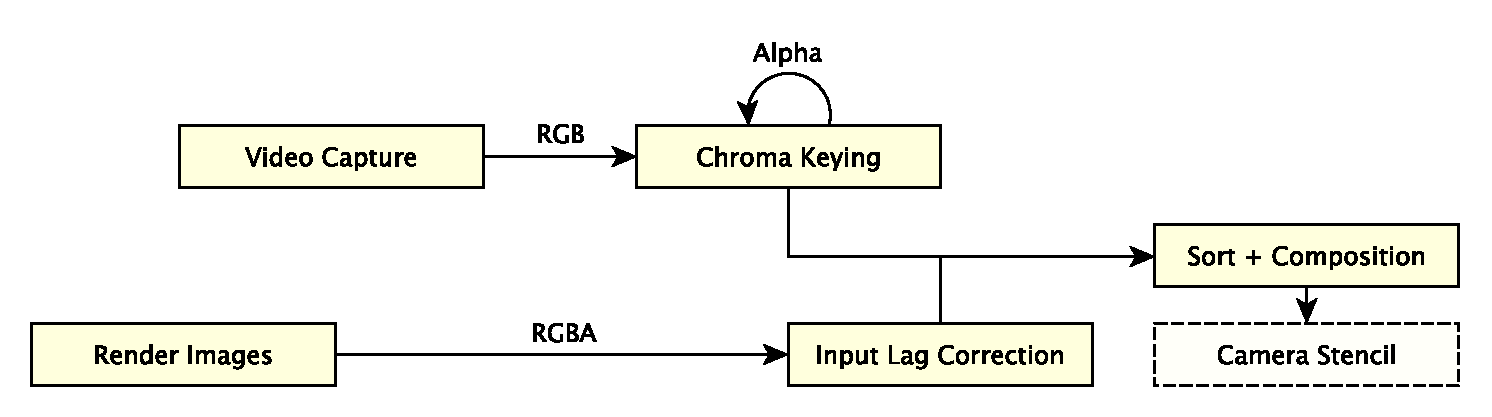
\includegraphics[width=\textwidth]{_raw_resources/pipeline_steps/4_6_stencil.pdf}
	\caption{After sorting the scene additional stenciling is necessary}
	\label{fig:steps:stencil}
\end{figure}

A virtual projection can be seen in figure \ref{fig:stencil:projection} with 
reconstructed camera parameters. With help of the engine-editor a greenscreen 
can be calibrated and should match very closely to all real world parameters, 
allowing a real world camera to film over the edges of a greenscreen without 
destroying the image composition. If a VR actor is outside of the chroma key 
planes, the resulting image composition wouldn't be usable, thus this solution 
enhances a resulting image without major drawbacks.

\begin{figure}[htbp]
	\caption{Virtual projection and photo of VR actor - note: in-engine 
	screenshot and photos were taken shortly apart and therefore don't fit 
	exactly}
	\label{fig:stencil:projection}
	\begin{subfigure}[t]{.45\textwidth}
		\centering
		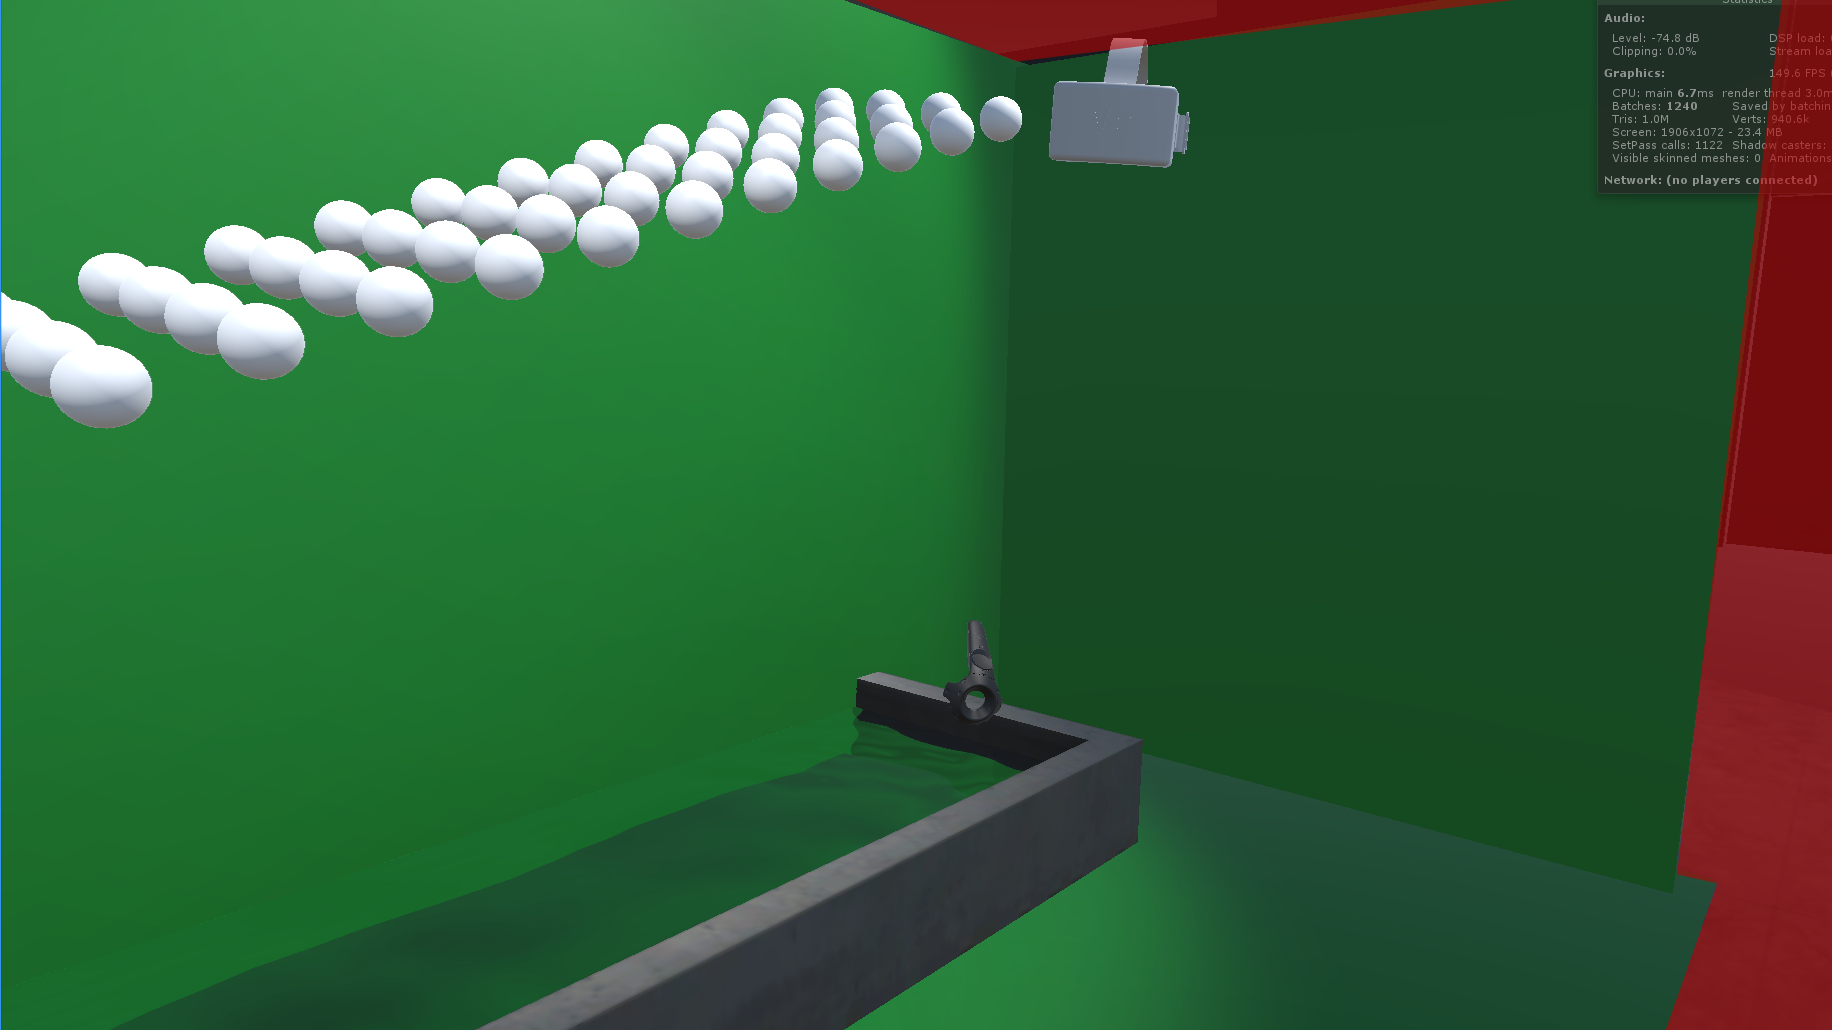
\includegraphics[width=\textwidth]{gfx/StencilProjection.png}
		\caption{Virtual reprojection of valid green screen - red colored areas 
		will be cut off}
	\end{subfigure}
	\begin{subfigure}[t]{.45\textwidth}
		\centering
		\includegraphics[width=\textwidth]{gfx/StencilCut.png}
		\caption{Masking what would be remaining video content - red colored 
		areas will be cut off}
	\end{subfigure}
\end{figure}

In-engine this setup is a simple addition: After registering another camera to 
the camera manager, it simply renders a green box. Taken from previous 
projection parameters in \ref{sec:projection-params} this virtual camera 
receives a dedicated culling mask which only contain all green box projection 
planes. All other cameras ignore this layer. After each drawn frame, Unity is 
able to clear the framebuffer with a color alpha as 0 - all remaining fragments 
from the green box write any color with an alpha as 1. This creates a lookup 
texture where an alpha-mask is created which will be transferred to the video 
feeds alpha.

Now we achieved a green box projection inside the same scene without using 
complex management processes with Unitys' scene manager. Due to the quick setup 
it works well for fast calibration and allows for a broad camera angle without 
degrading the mixed reality performance.
\newline
Unfortunately stencil-opertions are poorly documented in Unity and add an 
overhead which cannot be measured from builtin profiler tools - as such it adds 
unknown performance costs and have not been used in this thesis.		  % additional camera masking
% !TeX spellcheck = en_US
% !TEX root = ../thesis-example.tex
%
\section{Light Environment Reproduction}

To conclude all rendering steps taken by now: We have successfully created an 
image composition with correct projection parameters, recalculated a planar 
depth, synchronized in-engine frames with the camera input lag and realigned 
the frame rate between both image generating systems and cut off all overshot 
pixels that were recorded outside of the green screen.

\begin{figure}[htb]
	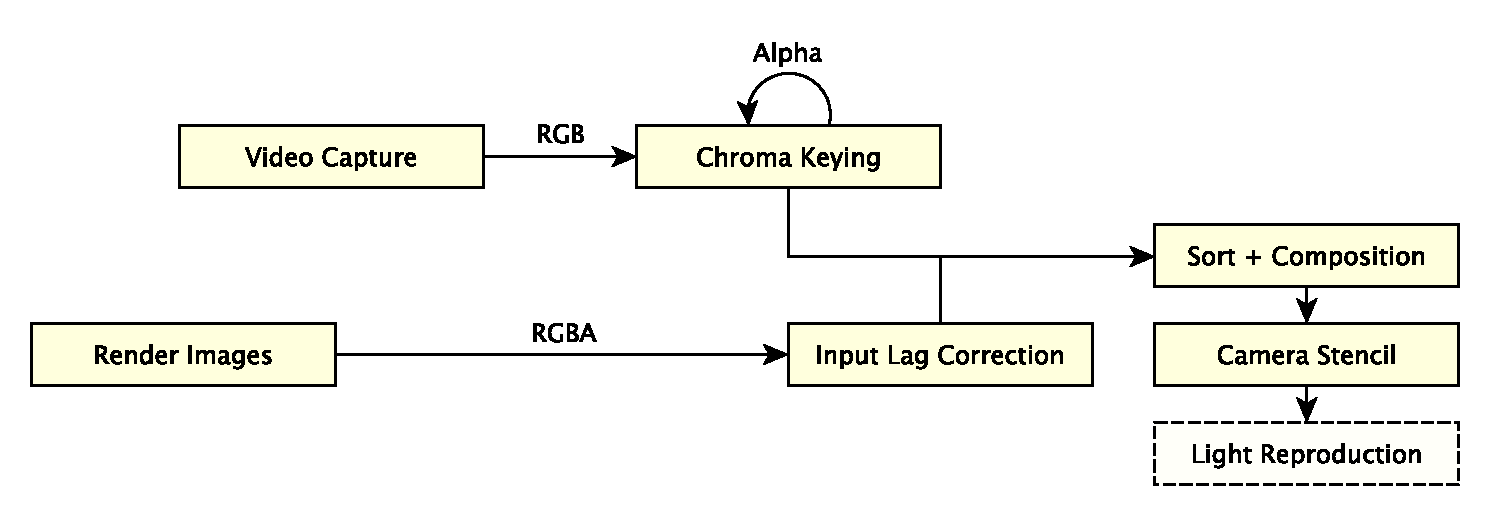
\includegraphics[width=\textwidth]{_raw_resources/pipeline_steps/4_7_lights.pdf}
	\caption{Following in this pipeline is lights reproduction}
	\label{fig:steps:lights}
\end{figure}

A minor last step is light-reproduction, in which an approximate lightning 
setting will be transferred from 3D environment to the video feed of a VR 
actor. Assuming that the video footage contains a natural lit, tint-free and 
calibrated video signal, it is possible to approximate how a VR actor would 
be lit like if he truly is inside the virtual environment.

\begin{figure}[htb]
	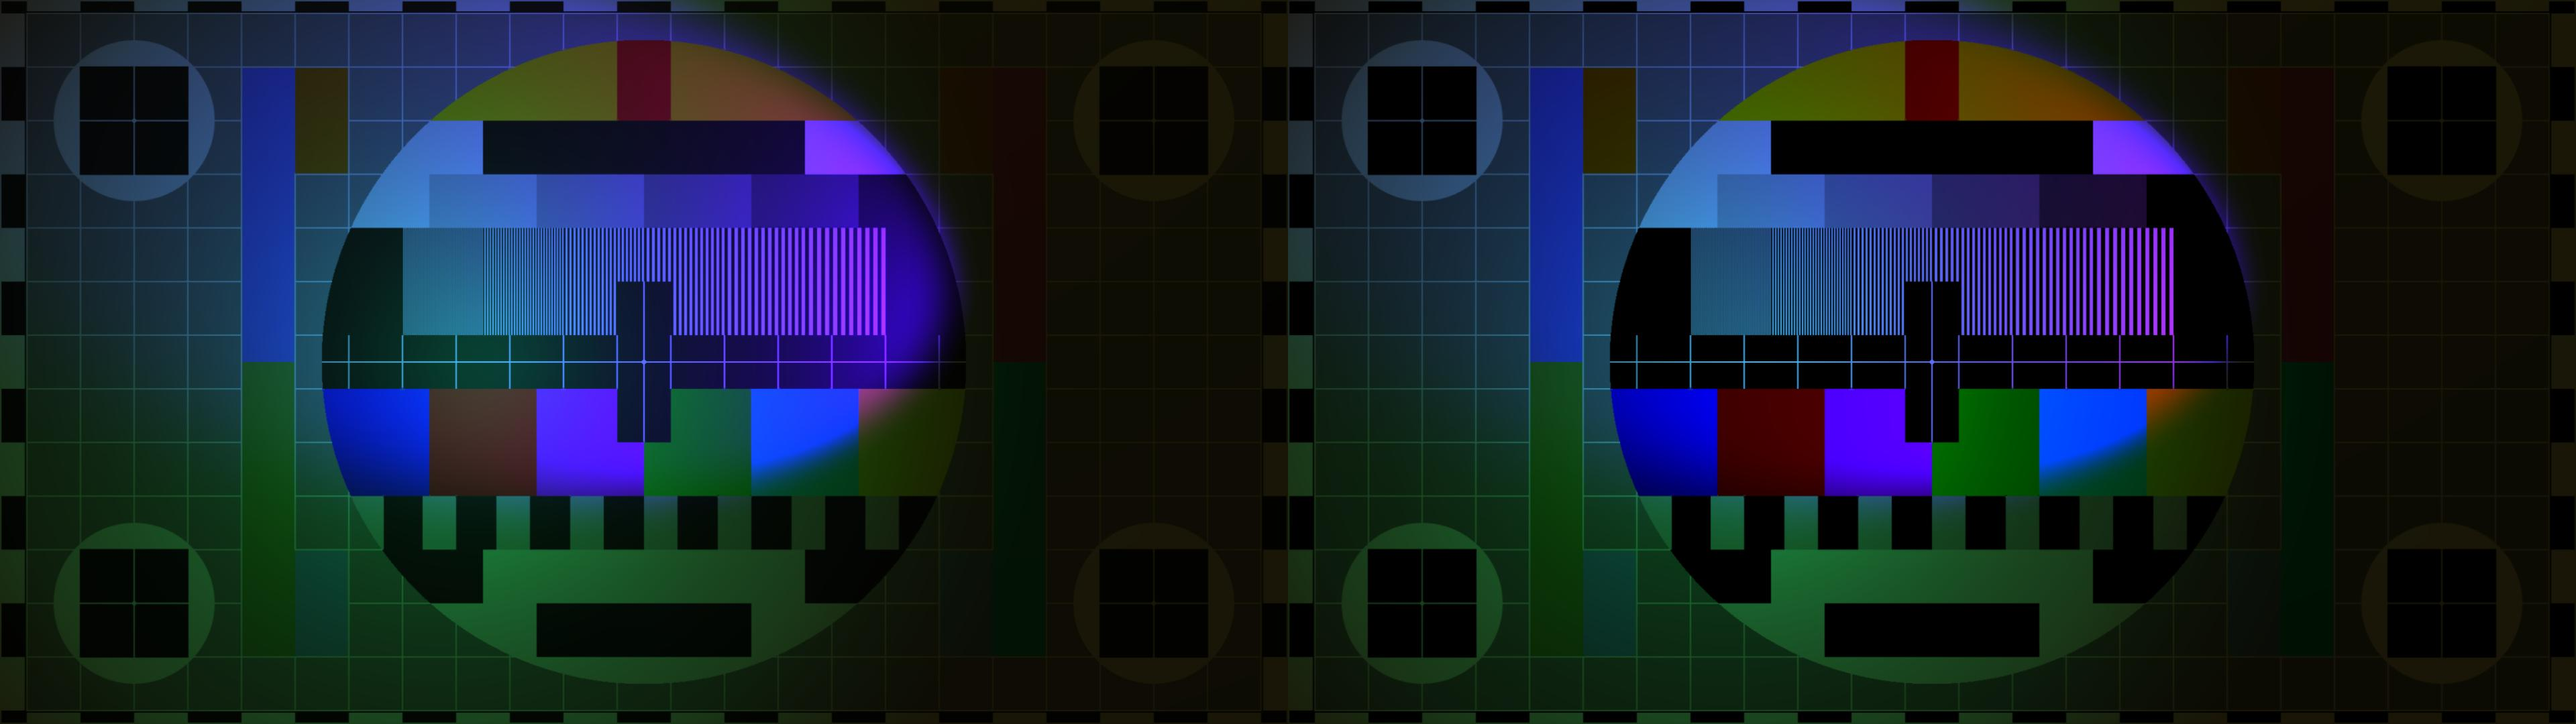
\includegraphics[width=\textwidth]{_raw_resources/light-reconstruction/comparison.jpg}
	\caption{Left: original, Right: reconstruction}
	\label{fig:light-reconstruction:comparison}
\end{figure}

Ambient light reproduction hinges on two assumptions: An actor's recorded video 
is flat for this purpose \textit{and} he receives clean and consistent light 
from all angles that has no additional glossiness. With that we can project a 
plane at the actor's position, filling the frustum edges of another virtual 
camera with the same camera projection parameters from section 
\ref{sec:projection-params}. This plane contains a simple lit material with 
white albedo coloring, which captures the lightning situation at this given 
point (figure \ref{fig:light-reconstruction:diff-capture} a).

To calculate the position $P_{pos}$ and size $\vec{P_{x, y}}$ with a 
given forward vector $\vec{C_{forward}}$ and position $C_{pos}$ of the 
camera, as well as a distance $Z$ between camera and actor and a current Field 
of View $FoV$ in radians by assuming a 16:9 video feed:

\eq{eq:light-reproduction:pos}{
	P_{pos} = C_{pos} + Z * \vec{C_{forward}}
}

\eq{eq:light-reproduction:size:1}{
	P_{x, y} =
	\begin{bmatrix}
		2 * \tan(FoV / 2) * Z \\
		P_{x} * \frac{16}{9}
	\end{bmatrix}	
}

These parameters can directly be applied to the transformation of said white 
plane which then captures the lightning environment inside the virtual scenes. 
As with all other composition-renderings, this step will be stored as a 
separate \code{RenderTexture} too and can operate on lower resolutions to speed 
up color and light sampling for performance gains.
\newline
The resulting frame buffer will be multiplied later onto the camera feed with a 
video color $C_V$ and the light plane $C_L$:

\eq{eq:light-reproduction:composition}{
	C_T = 
	\begin{bmatrix}
		C_{V_R} * C_{L_R} \\
		C_{V_G} * C_{L_G} \\
		C_{V_B} * C_{L_B}
	\end{bmatrix}
}

Lastly, a directional light with the same culling mask can be applied, to 
improve the overall brightness of this light mask to allow for more natural 
tint than a linear color operation.

\begin{figure}[htbp]
	\caption{A comparison of different composition methods in engine}
	\label{fig:light-reconstruction:diff-capture}
	\begin{subfigure}[t]{.45\textwidth}
		\centering
		
\includegraphics[width=\textwidth]{gfx/recoloring/plane.png}
		\caption{captured, lit plane}
	\end{subfigure}
	\begin{subfigure}[t]{.45\textwidth}
		\centering
		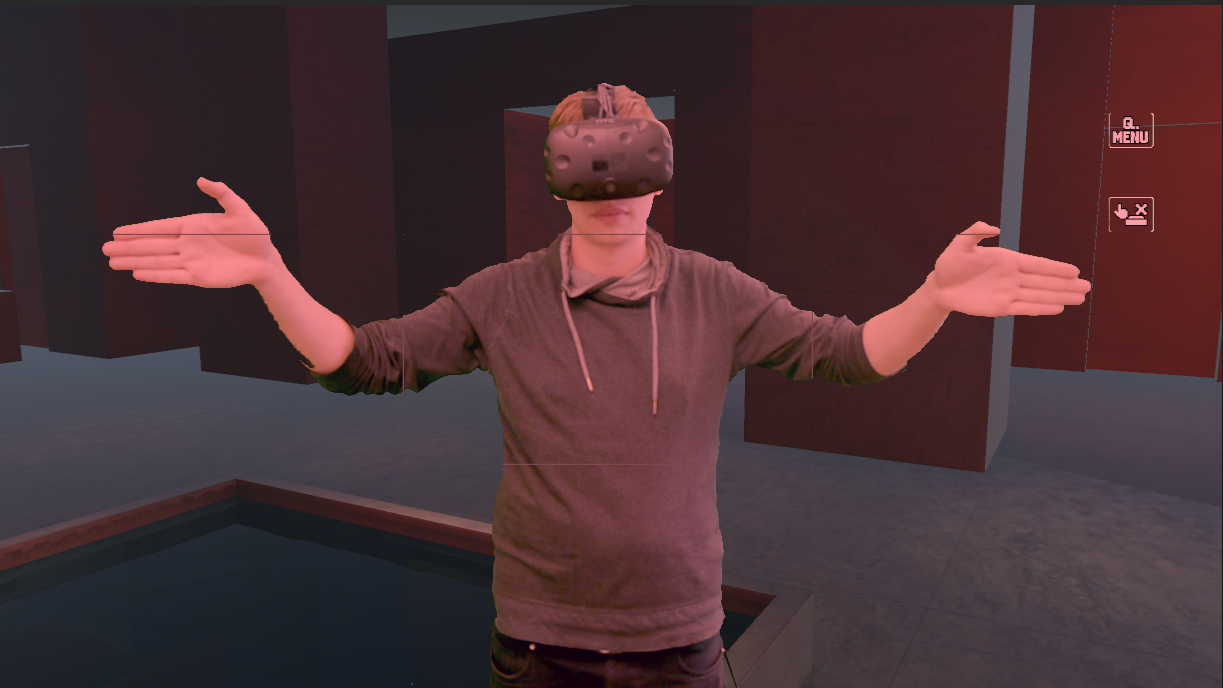
\includegraphics[width=\textwidth]{gfx/recoloring/img.png}
		\caption{Light plane applied to the actor}
	\end{subfigure}
\end{figure}

\todo[inline]{margin of error of light reproduction}
        % Light reproduction
% !TeX spellcheck = en_US
% !TEX root = ../thesis-example.tex
%
\section{Additional Coloring Operations}

Finally, we have created the best possible recreation of a VR actor inside the 
virtual reality scene. Now we can follow up with post effects on the video feed 
to fit it better into the environment.

\begin{figure}[htb]
	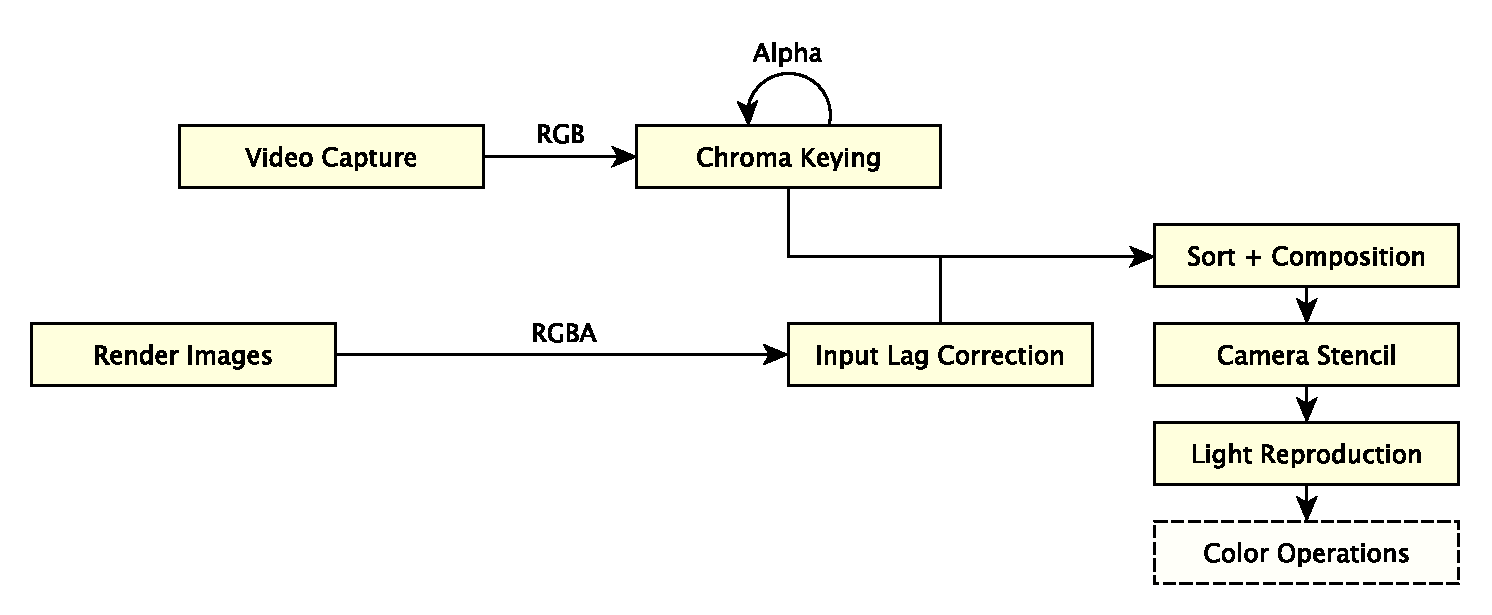
\includegraphics[width=\textwidth]{gfx/pipeline/4_8_color.pdf}
	\caption{Initial step upon receiving the camera image}
	\label{fig:steps:recolor}
\end{figure}

This can be done with regular coloring operations, like hue rotation, 
brightness, contrast and saturation procedures on the video alone. It gives a 
content producer direct enhancing tools which would be usually given by Unity's 
post effects stack, which are unavailable due to the nature of this render 
pipeline.

\subsection{Color Spill Removal \& Recoloring}

The green box as background spills --- so to say --- its green color on the 
actor to a certain degree. With proper lightning setups\footnote{A example 
setup can be found in the Appendix \ref{app:lightningsetup}} it is possible to 
mitigate this effect but color retouching is in almost all cases a necessity. 
\textbf{YCgCo} is, again, good enough to perform this color operation, thanks 
to its color decoupling properties and a green chrominance channel. By 
splitting a RGB image into YCgCo $C_{Input}$ (see equation 
\eqref{eq:ycgco:transformation}) and then shifting towards the complementary 
color of a given key color $C_{Key}$ for a factor weight $W \in [0, 1]$:

\eq{eq:retouch:spill:1}{
	R = \frac{C_{Key Cg, Co} \cdot C_{Input Cg, Co}}{C_{Key Cg, Co} \cdot 
	C_{Key Cg, Co}}
}

\eq{eq:retouch:spill:2}{
	\begin{bmatrix}
		Y  \\
		Cg \\
		Co \\
	\end{bmatrix}
	= 
	\begin{bmatrix}
		Y \\
		C_{Key Cg} * (R + 0.5) * W \\
		C_{Key Co} * (R + 0.5) * W
	\end{bmatrix}
}

Since this is a linear operation, it does not consider more apparent color 
spill around an actor's edges --- it slightly removes a green undertone to make 
the video image look more natural and fitting into a scene.

Additionally, we can apply a hue color rotation by using Rodrigues' rotation 
formula to make changes to the overall tint of an 
image\cite{shagam:hsv-rotation}. With that we can achieve a more natural 
looking video feed that integrates well into any given scene. Allowing for 
color-shifting degrades the signal but allows --- if needed --- for a more 
fitting composition between an actor and his surrounding virtual reality 
scenery.

\subsection{Brightness, Contrast and Saturation}

Additionally, to give a user full control over image composition, we have a 
brief look at other linear image transformations to give good control over the 
video feed, which are brightness, contrast and saturation operations:

Brightness increases all color channels of a given color $C_I$ for a brightness 
factor of $F_B$:

\eq{eq:retouch:brightness}{
	C_T =
	\begin{bmatrix}
		C_{I_R} + F_B \\
		C_{I_G} + F_B \\
		C_{I_B} + F_B
	\end{bmatrix}
}

Contrast is a color multiplication in which the input color $C_I$ will be 
decreased by half of a channels maximum value, multiplied by a contrast factor 
$F_C$ and increased by half a maximum channels color again:

\eq{eq:retouch:contrast}{
	C_T =
	\begin{bmatrix}
		(C_{I_R} - 0.5) * F_B + 0.5 \\
		(C_{I_G} - 0.5) * F_B + 0.5 \\
		(C_{I_B} - 0.5) * F_B + 0.5
	\end{bmatrix}
}

Saturation is done by calculating the color intensity $I$ and then mixing these 
both colors for a saturation factor $F_S$:

\eq{eq:retouch:saturation:1}{
	I_{R, G, B} =
	\begin{bmatrix}
		C_{I_R} * 0.2126 \\
		C_{I_G} * 0.7152 \\
		C_{I_B} * 0.0722
	\end{bmatrix}
}

And $Lerp(x, y, t)$ being defined as:

\eq{eq:retouch:saturation:2}{
	Lerp(a, b, t) = a (1 - t) + b t
}

\eq{eq:retouch:saturation:3}{
	C_T = 
	\begin{bmatrix}
		Lerp(C_{I_R}, I_R, F_S) \\
		Lerp(C_{I_G}, I_G, F_S) \\
		Lerp(C_{I_B}, I_B, F_S)
	\end{bmatrix}
}
       % additional color operations
% !TeX spellcheck = en_US
% !TEX root = ../thesis-example.tex
%
\section{Closing remark: order of calculation}

The discussed order is written in respect of transformation operations from an 
incoming feed, in reality an optimized pipeline is changed slightly. In 
example, post processing the video feed has to be done before it is composited 
into the mixed reality image. This flowchart (\ref{fig:steps:order:alt}) 
demonstrates the actual calculation sequence. Also shown is a separation 
between engine scripting and shader programming.

\begin{figure}[htb]
	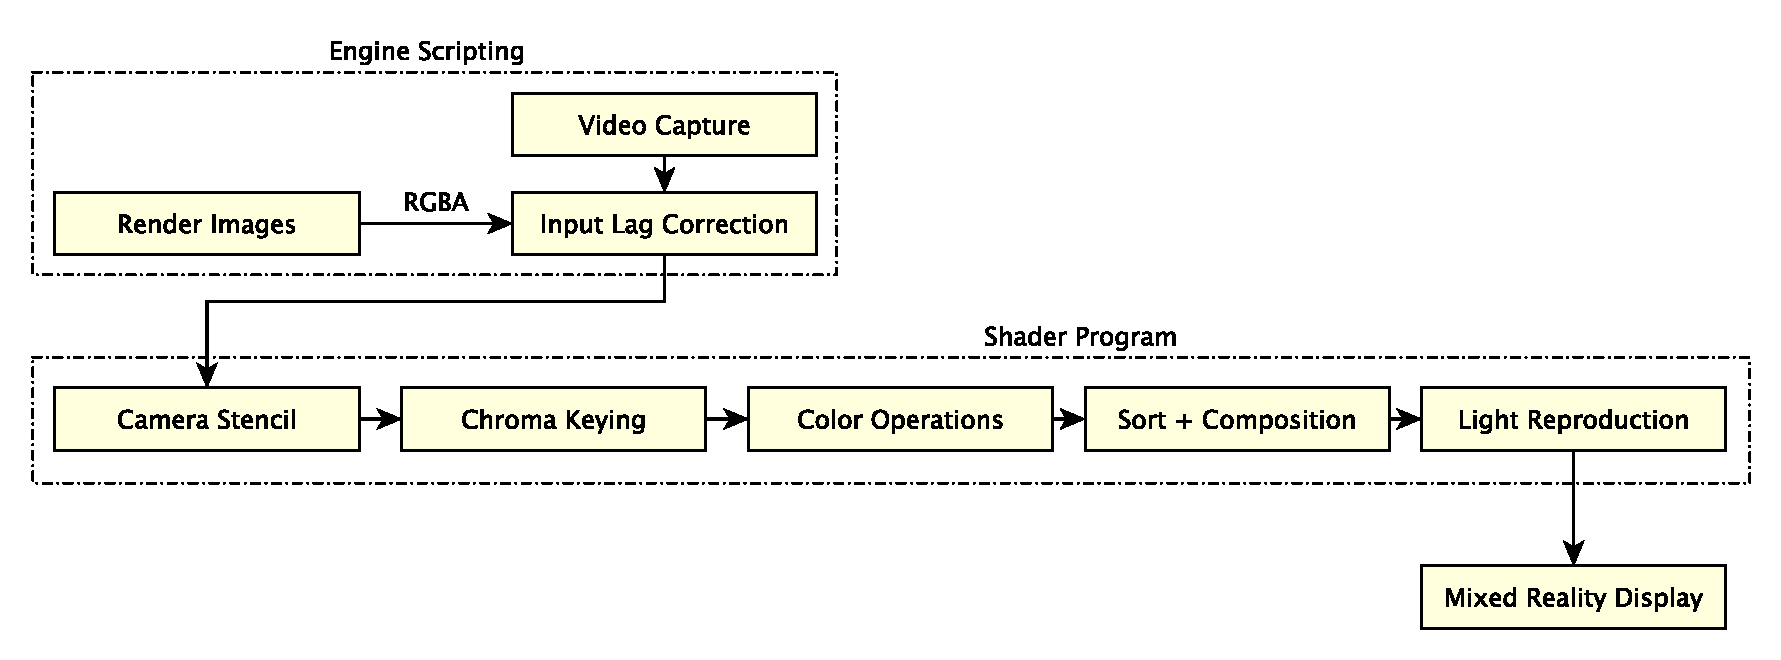
\includegraphics[width=\textwidth]{_raw_resources/pipeline_steps/4_9_order_alt.pdf}
	\caption{Actual order of computation}
	\label{fig:steps:order:alt}
\end{figure}

\todo[inline]{This might be appendix-worthy - then move a note to the chapters' 
beginning.}			  % order of calculation